%%%%%%%%%%%%%%%%%%%%%%%%%%%%%%%%%%%%%%%%%
% University Assignment Title Page 
% LaTeX Template
% Version 1.0 (27/12/12)
%
% This template has been downloaded from:
% http://www.LaTeXTemplates.com
%
% Original author:
% WikiBooks (http://en.wikibooks.org/wiki/LaTeX/Title_Creation)
%
% License:
% CC BY-NC-SA 3.0 (http://creativecommons.org/licenses/by-nc-sa/3.0/)
% 
% Instructions for using this template:
% This title page is capable of being compiled as is. This is not useful for 
% including it in another document. To do this, you have two options: 
%
% 1) Copy/paste everything between \begin{document} and \end{document} 
% starting at \begin{titlepage} and paste this into another LaTeX file where you 
% want your title page.
% OR
% 2) Remove everything outside the \begin{titlepage} and \end{titlepage} and 
% move this file to the same directory as the LaTeX file you wish to add it to. 
% Then add \input{./title_page_1.tex} to your LaTeX file where you want your
% title page.
%
%%%%%%%%%%%%%%%%%%%%%%%%%%%%%%%%%%%%%%%%%
%\title{Title page with logo}
%----------------------------------------------------------------------------------------
%	PACKAGES AND OTHER DOCUMENT CONFIGURATIONS
%----------------------------------------------------------------------------------------

\documentclass[11pt]{article}
\usepackage[english]{babel}
\usepackage[utf8x]{inputenc}
\usepackage{amsmath}
\usepackage{graphicx}
\usepackage[colorinlistoftodos]{todonotes}
\usepackage[a4paper,bindingoffset=0.2in,%
            left=0.3in,right=0.5in,top=1in,bottom=1in,%
            footskip=.25in]{geometry}
            \usepackage{multicol}
\newenvironment{Figure}
 {\par\medskip\noindent\minipage{\linewidth}}
{\endminipage\par\medskip}
\begin{document}

\begin{titlepage}

\newcommand{\HRule}{\rule{\linewidth}{0.5mm}} % Defines a new command for the horizontal lines, change thickness here

\center % Center everything on the page

%----------------------------------------------------------------------------------------
%	HEADING SECTIONS
%----------------------------------------------------------------------------------------

\textsc{\LARGE Università degli studi di Milano-Bicocca}\\[1cm] % Name of your university/college
\textsc{\Large High Dimensional Data Analysis}\\[0.3cm] % Major heading such as course name
\textsc{\large }\\[0.1cm] % Minor heading such as course title

%----------------------------------------------------------------------------------------
%	TITLE SECTION
%----------------------------------------------------------------------------------------

\HRule \\[0.4cm]
{ \huge \bfseries Linking Long-Term Dietary Patterns with Gut Microbial Enterotypes}\\[0.4cm] % Title of your document
\HRule \\[1.5cm]
 
%----------------------------------------------------------------------------------------
%	AUTHOR SECTION
%----------------------------------------------------------------------------------------

\large
\emph{Authors:}\\
Lorenzo Camaione - 850380- l.camaione@campus.unimib.it \\   % Your name
Martino Lorenzo Tenconi - MTS4128991- m.tenconi3@campus.unimib.it \\  % Your name
Lorenzo Famiglini - MTS4128991- l.famiglini@campus.unimib.it   \\[1cm] % Your name

% If you don't want a supervisor, uncomment the two lines below and remove the section above
%\Large \emph{Author:}\\
%John \textsc{Smith}\\[3cm] % Your name

%----------------------------------------------------------------------------------------
%	DATE SECTION
%----------------------------------------------------------------------------------------

{\large \today}\\[2cm] % Date, change the \today to a set date if you want to be precise

%----------------------------------------------------------------------------------------
%	LOGO SECTION
%----------------------------------------------------------------------------------------


\includegraphics{figs/logo.png}\\[1cm] % Include a department/university logo - this will require the graphicx package
 
%----------------------------------------------------------------------------------------

\vfill % Fill the rest of the page with whitespace

\end{titlepage}


\begin{abstract}
Nell'articolo sono riportati i risultati e le metodologie di analisi di uno studio che ha avuto l'obiettivo di replicare quello descritto nel paper \cite{paper}. Lo scopo è quello di verificare l'associazione tra nutrienti e microbioma ed infine fornire un modello di previsione del BMI in funzione di batteri del microbioma, nutrienti ed altri fattori demografici quali età e sesso. Della fase di preprocessing hanno fatto parte l'applicazione della permanova sulle distanze unifrac tra individui ed il metodo FDR. Oltre alle analisi delle componenti principali sono stati analizzati i seguenti modelli: modello lineare con stepwise selection e modello lasso. 
L'associazione tra nutrienti e batteri è risultata forte mentre si è verificato che il BMI è fortemente influenzato dalla diversa composizione batterica oltre che dall'età e dal sesso di una persona. 
\end{abstract}

\section{Introduction}
La dieta influenza significativamente la salute umana ed in parte anche il microbioma dell’intestino. In questo studio, da un campione di 97 persone, sono stati estratti dati sulla dieta e sulla composizione del DNA delle loro feci. I batteri presenti nelle feci possono essere clusterizzati in enterotipi che differiscono tra loro perlopiù per i livelli di Bacteroides e Prevotella. Inoltre, questi enterotipi possono essere associati a diete assunte per un lungo periodo. In particolare alti livelli di Bacteroides possono essere associati a diete ricche di proteine e grasso animale mentre alti livelli di Prevotella con carboidrati. 
Oltre ad analizzare l’associazione dieta-enterotipo si sono anche studiati dei modelli che spiegano il livello di BMI in funzione di nutrienti, microbioma e fattori demografici.

\section{Datasets}
I dataset a disposizione per le analisi sono forniti dal portale QIITA (study ID 1011) e sono rappresentati da una tabella OTU, una tavola tassonomica e un questionario FFQ relativo ai nutrienti assunti dai soggetti nella dieta a lungo termine. La tabella OTU, di dimensioni 3393 x 100, contiene il numero di sequenze che sono state osservate per ognuno dei 3393 batteri presenti nel microbioma di ciascuno dei 100 pazienti. Ognuno dei batteri può essere presente o assente nel microbioma di ogni paziente e la combinazione di questi valori determina il microbioma vero e proprio di ciascun paziente. La tavola tassonomica permette di collegare gli identificativi dei batteri presenti nella tabella OTU alle loro tassonomie; in questa tavola sono indicati per ognuno dei 3393 batteri i sette livelli tassonomici regno, phylum, classe, ordine, famiglia, genere e specie. Infine il questionario dei nutrienti contiene, per 98 soggetti, le quantità di ciascuno dei nutrienti assunti in una dieta di lungo periodo. In aggiunta a questi tre dataset vi è una quarta tabella contenente gli id dei 100 soggetti in studio e una serie di variabili, come ad esempio il genere, l’altezza, il peso, l’età e il Body Mass Index (BMI) a loro associate. Le informazioni estratte da questo ultimo dataset, combinate con le variabili estratte nella fase di preprocessing, saranno utilizzate per scopi di analisi predittiva del BMI.

\subsection{Preprocessing}
Si è effettuata una prima pulizia della tavola tassonomica rimuovendo caratteri speciali dai nomi delle tassonomie e si sono analizzate quindi la tavola e le osservazioni per ciascuna colonna indicante il livello tassonomico. Poiché lo studio\cite{paper} è improntato all’analisi dei batteri a livello di genere, ci si concentra sull’analisi delle variabili indicanti i nomi delle tassonomie fino al sesto livello, ignorando la specie dei batteri osservati. La tavola tassonomica presenta un totale di 1526 batteri con genere non identificato e dunque ai fini della analisi si considerano per questi batteri i soli livelli precedenti presenti; ad esempio per un batterio che ha classificazione fino al quarto livello (“ordine”) si considerano unicamente le prime quattro tassonomie eliminando quindi i valori mancanti per i successivi livelli. A questo punto vengono raggruppati tra loro i batteri nella tabella OTU che hanno la stessa classificazione fino all’ultimo livello presente; si ottengono quindi cinque dataset, ognuno per ogni livello tassonomico da phylum a genere, contenenti le possibili aggregazioni osservate per il relativo livello. Per ognuna di queste cinque tabelle sono calcolate le abbondanze relative dei batteri, ovvero la presenza in termini percentuali di ciascun batterio in ognuno dei 100 individui considerati. Aggregando queste cinque tabelle si ottengono 198 possibili livelli di aggregazione dei batteri osservati. Sono state considerate, in seguito, solamente le tassonomie presenti in almeno il 10\% dei soggetti che avessero un valore di abbondanza relativa maggiore o uguale allo 0.2\% in almeno uno dei soggetti. In questo modo sono state ottenute 76 tassonomie.
Inoltre, per scopi successivi nelle analisi, si decide di creare una tabella OTU contenente i batteri aggregati al solo livello di genere o superiore ove mancante (famiglia, genere, classe, …), ottenendo così 119 tassonomie differenti. 
Si mostrano le abbondanze nei 97 pazienti dei generi di batteri osservati:


\vspace*{1cm}
\begin{Figure}
    \centering
    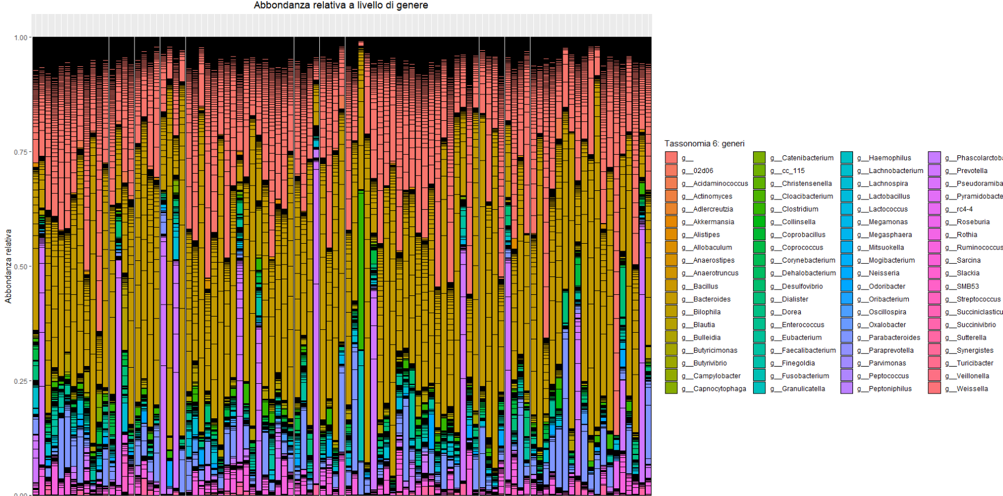
\includegraphics[width=\linewidth,keepaspectratio]{images/abbondanza-generi.png}
  \end{Figure}
 \vspace*{1cm}  

Per quanto riguarda il dataset dei nutrienti, di dimensione 98 x 215, sono state selezionate soltanto le 97 righe con identificativo del soggetto nello studio presente anche nella tabella OTU citata in precedenza. 
Per valutare quali nutrienti fossero maggiormente significativi a livello di impatto sulla composizione del  intestinale, è stata considerato l’intero insieme dei 3393 diversi batteri non aggregati per livello tassonomico come indicatore di variabilità della composizione del microbioma stesso. Sulle abbondanze della tabella OTU originaria sono state dunque calcolate le distanze tra i microbiomi intestinali dei 97 soggetti con la metrica Unifrac \cite{unifrac} non pesata, individuata come metodo maggiormente discriminante per le differenze di composizione dei microbiomi rispetto alla stessa metrica Unifrac pesata, che tiene quindi in considerazione la quantità di ciascun batterio nel microbioma, piuttosto che la semplice presenza/assenza come nel caso della metrica non pesata. Il calcolo della distanza utilizzando la Unifrac non pesata avviene tramite la formula: 
$$\frac{sum\: of \:unshared \:branch\: lengths}{sum\: of\: all\: tree\: branch\: lengths} = fraction\: of\: total \:unshared \:branch \:lengths$$

Una volta calcolata la matrice delle distanze non pesate Unifrac sui 97 microbiomi intestinali, è stato possibile effettuare la PERMANOVA\cite{permanova} su ciascuno dei nutrienti standardizzati della tabella. A differenza della ANOVA, che si basa sull’ipotesi di normalità, la PERMANOVA traccia test di significatività confrontando il risultato del test F reale con quello ottenuto dalle permutazioni casuali degli oggetti tra i gruppi senza fare alcuna assunzione sulla distribuzione dei dati; inoltre, mentre l'ANOVA verifica la somiglianza delle medie tra i gruppi basandosi sui dati, la PERMANOVA utilizza in input una matrice di distanze. Ognuno dei nutrienti è stato valutato significativo se il valore di False Discovery Rate FDR (percentuale di volte in cui si rifiuta l’ipotesi nulla quando invece è vera) è minore del 25\%. Come descritto in ***ref***, questa soglia relativamente alta è stata utilizzata per non escludere dall’analisi nutrienti associati a batteri con valori di abbondanza relativa non particolarmente alti.
I batteri e i nutrienti selezionati sono stati utilizzati per costruire due dataset con lo scopo di effettuare l’analisi predittiva del BMI. Dai nutrienti selezionati sono state estratte le prime 5 componenti principali per un totale di varianza catturata del 70\%. Nel primo dataset sono state inserite le 119 tassonomie rilevanti e le loro relative componenti principali con un 80\% di varianza catturata. Nel secondo dataset sono state inserite solamente le 37 tassonomie a livello di genere, senza considerare potenziali livelli superiori. I dataset utilizzati per l’analisi predittiva sono stati suddivisi in training e test: la parte dedicata all’addestramento dei modelli è risultata essere il 90\%, lasciando il 10\% dei dati per la validazione dei modelli.


\section{Analisi descrittiva}
Nella heatmap seguente si mostrano le correlazioni di Spearman ottenute tra i generi estratti dalle 76 tassonomie rilevanti e i nutrienti selezionati con la PERMANOVA. 
Dalla heatmap delle correlazioni è evidente come le proteine come arginina, alanina, glicina e leucina siano correlate positivamente con il genere Bacteroides, mentre risulta debole e negativa la correlazione di tali nutrienti con i due generi Prevotella osservati nei microbiomi dei soggetti in studio. D’altra parte Prevotella mostra un'alta correlazione positiva con nutrienti ricchi di zuccheri, come saccarosio, fruttosio, carboidrati e indice glicemico; la quantità relativa di Bacteroides nel microbioma intestinale risulta invece poco correlata con i carboidrati. Per quanto riguarda le fibre e per i composti di origine vegetale invece non si mostra forte correlazione per nessuno dei due generi presi in esame. Il terzo genere preso in considerazione in studi precedenti [link a studi precedenti], Ruminococcus, risulta invece correlato positivamente con questa ultima categoria di nutrienti. Tuttavia, la sua correlazione risulta debole e negativa sia per quanto riguarda i nutrienti riconducibili ai carboidrati, sia per gli amminoacidi.
\\
\begin{Figure}
    \centering
    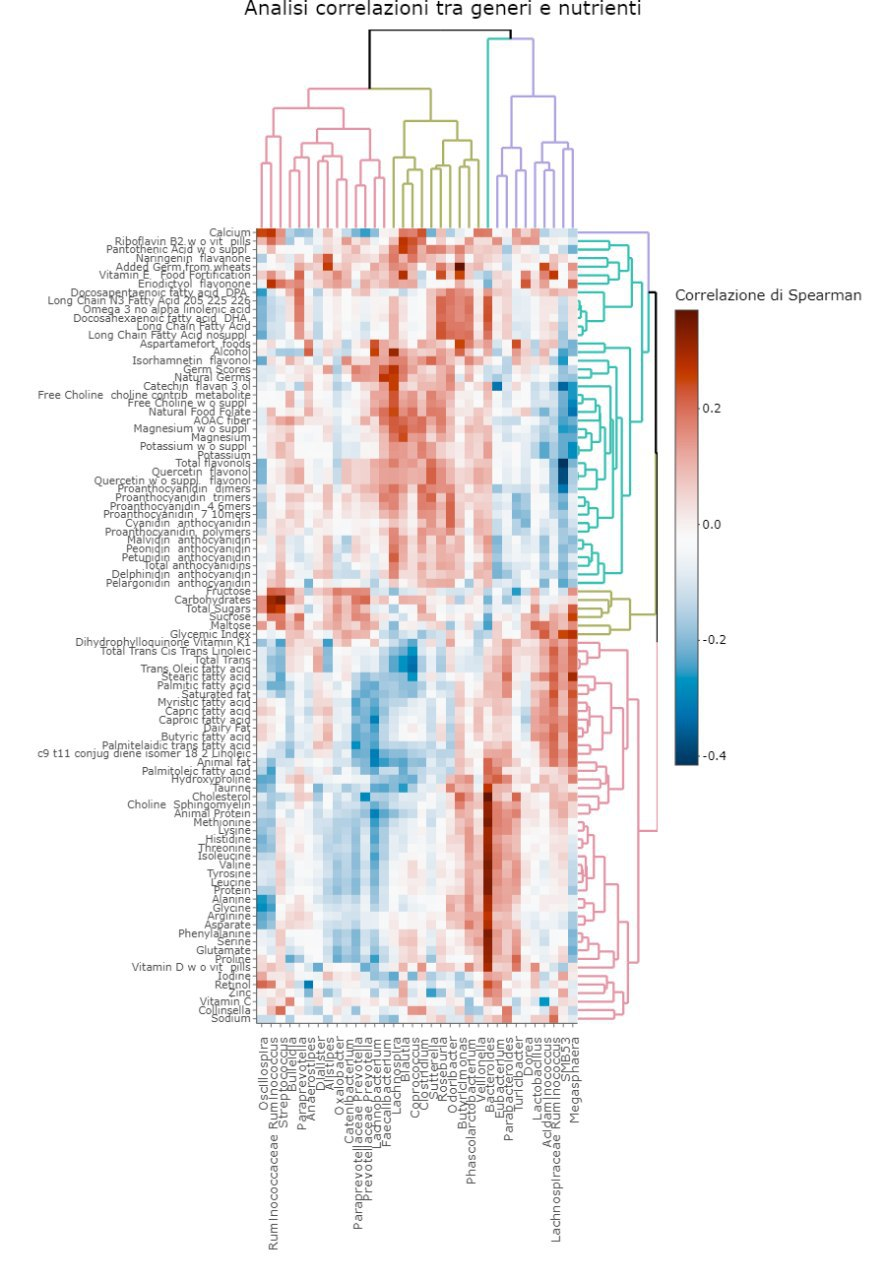
\includegraphics[width=\linewidth,keepaspectratio]{images/real_correlazione.jpeg}
  \end{Figure}

Successivamente si è utilizzata la aggregazione dei batteri nelle 119 tassonomie a livello di genere per effettuare un raggruppamento delle composizioni dei microbiomi in clusters. Come suggerito da \cite{paper}, si è effettuato un clustering PAM (Partitioning Around Medoid).
Sono state provate tre differenti metriche di distanza, ovvero la distanza euclidea, la dissimilarità di Bray-Curtis, fortemente utilizzata in ambito biologico e infine la Jensen-Shannon divergence JSD \cite{jsd}. In tutti e tre i casi il numero ottimale di cluster da considerare è stato 2, a cui sono associati i coefficienti di Silhouette maggiori. 

\begin{Figure}
\begin{multicols}{2}
    \centering
         \vspace*{1.7cm}
     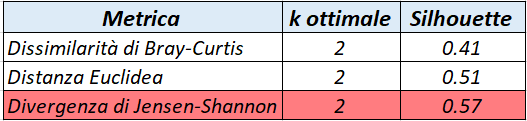
\includegraphics[width=8cm,keepaspectratio, scale=0.3]{images/real_tabella.PNG}
    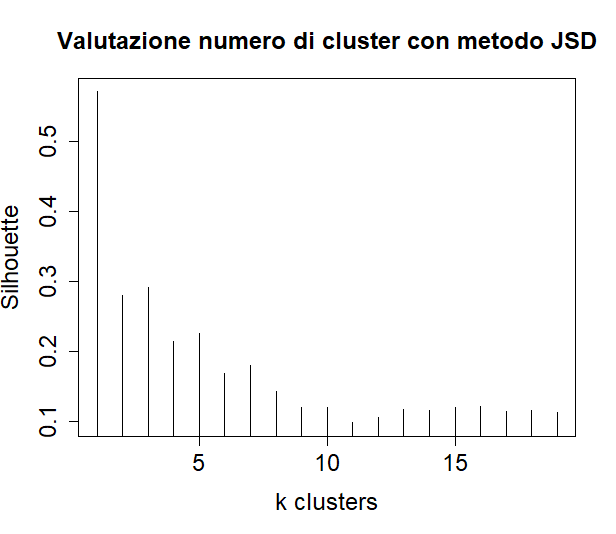
\includegraphics[width=\linewidth,keepaspectratio]{images/silhouette.png}
     \end{multicols}
  \end{Figure}

  
Poiché presenta il maggiore coefficiente di Silhouette, e dunque la massima diversità tra gruppi e massima coesione all’interno di essi, si è scelto il clustering calcolato mediante la matrice delle distanze con metrica JSD. 
Sulla stessa matrice delle distanze JSD sono state estratte le prime due componenti principali utilizzando la tecnica PCoA che, a differenza della PCA, accetta in input una matrice delle distanze invece che la matrice dei dati. In figura si possono vedere le osservazioni rappresentate nel piano delle prime due componenti principali, che spiegano rispettivamente il 40.2\% e il 17.3\% della variabilità dei batteri considerati.
\begin{Figure}
    \centering
    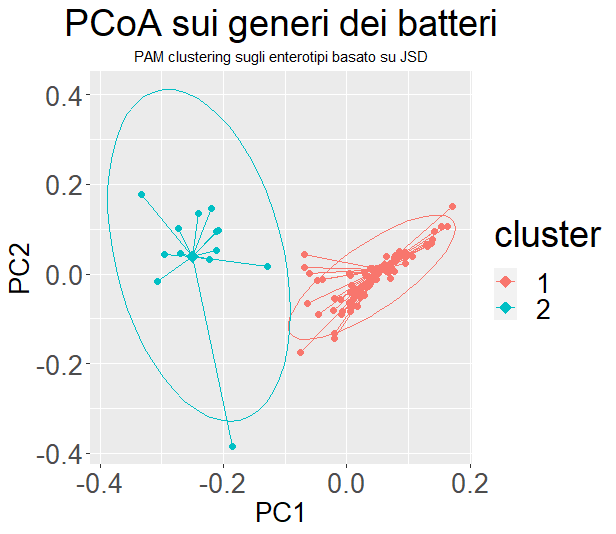
\includegraphics[width=\linewidth/2,keepaspectratio]{images/real_clustering.png}
  \end{Figure}

Osservando le composizioni dei due diversi cluster, si nota una netta differenziazione in termini di abbondanza dei generi Bacteroides e Prevotella. Mentre il cluster 1, rappresentato da soli 14 individui, registra un’alta abbondanza di Prevotella e un'abbondanza di Bacteroides prossima allo zero, il secondo raggruppamento ha comportamento esattamente opposto: in esso risiede una maggiore concentrazione di Bacteroides a scapito di una presenza del genere Prevotella molto ridotta.
Si è investigata inoltre la possibile rilevanza della presenza di Ruminococcus all’interno dei due cluster ottenuti, per verificare se la concentrazione di questo genere di batterio avesse una qualche influenza nella composizione del cluster. Si è osservato tuttavia che Ruminococcus si distribuiva in egual modo nei due gruppi, suggerendo una scarsa capacità di discriminazione degli enterotipi ottenuti.
\\
\vspace*{1cm}
\begin{Figure}
	\begin{multicols}{3}
    \centering
    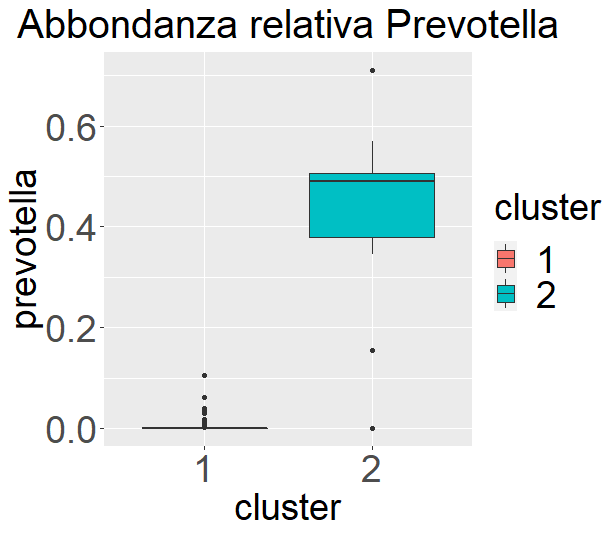
\includegraphics[width=\linewidth,keepaspectratio]{images/real_prevotella.png}
        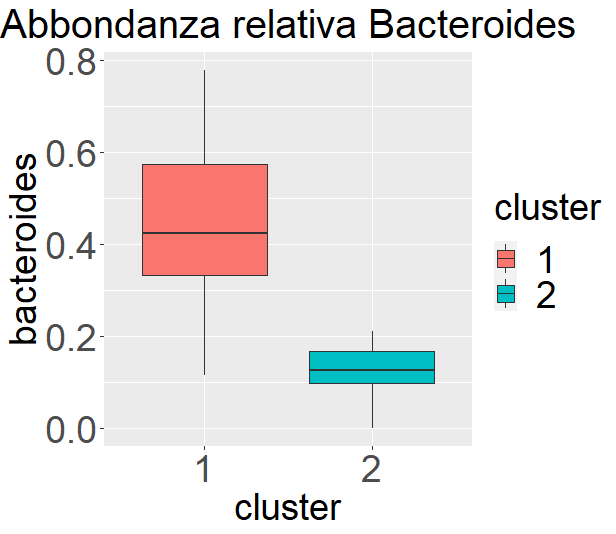
\includegraphics[width=\linewidth,keepaspectratio]{images/real_bacteroides.png}
                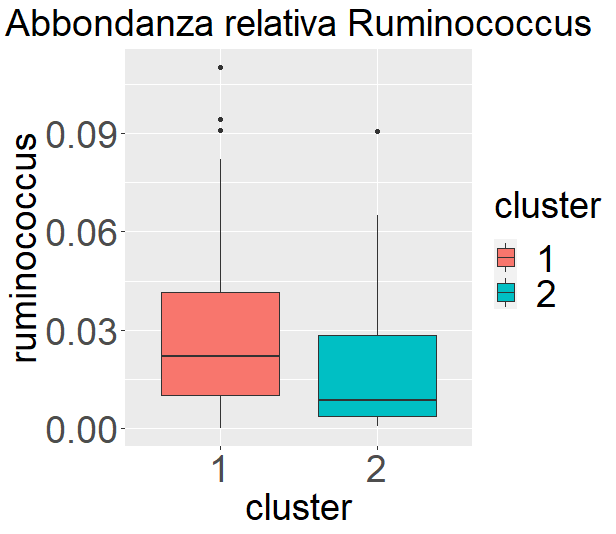
\includegraphics[width=\linewidth,keepaspectratio]{images/real_ruminococcus.png}
        \end{multicols}
  \end{Figure}
 \vspace*{1cm}
Infine, per ognuno dei due enterotipi, sono state valutate le associazioni con i nutrienti selezionati in precedenza. L’associazione è stata calcolata come la media dei nutrienti standardizzati all’interno dei due differenti gruppi.
In generale si osserva in maniera netta un'associazione forte dell’enterotipo 2 (Prevotella) con carboidrati, zuccheri e glucosio. Questa associazione risulta invece essere opposta per diete ricche di colesterolo, grassi e proteine animali. L’enterotipo 1, caratterizzato da una maggiore presenza di Bacteroides, risulta invece debolmente associato ma in maniera positiva con nutrienti riconducibili ad amminoacidi, proteine e grassi animali. L’associazione diminuisce quando dal gruppo delle proteine e dei grassi animali si passa a quelli delle fibre, vegetali e tutti quei nutrienti ricchi di zuccheri fino a diventare negativa.\\
\begin{Figure}
    \centering
    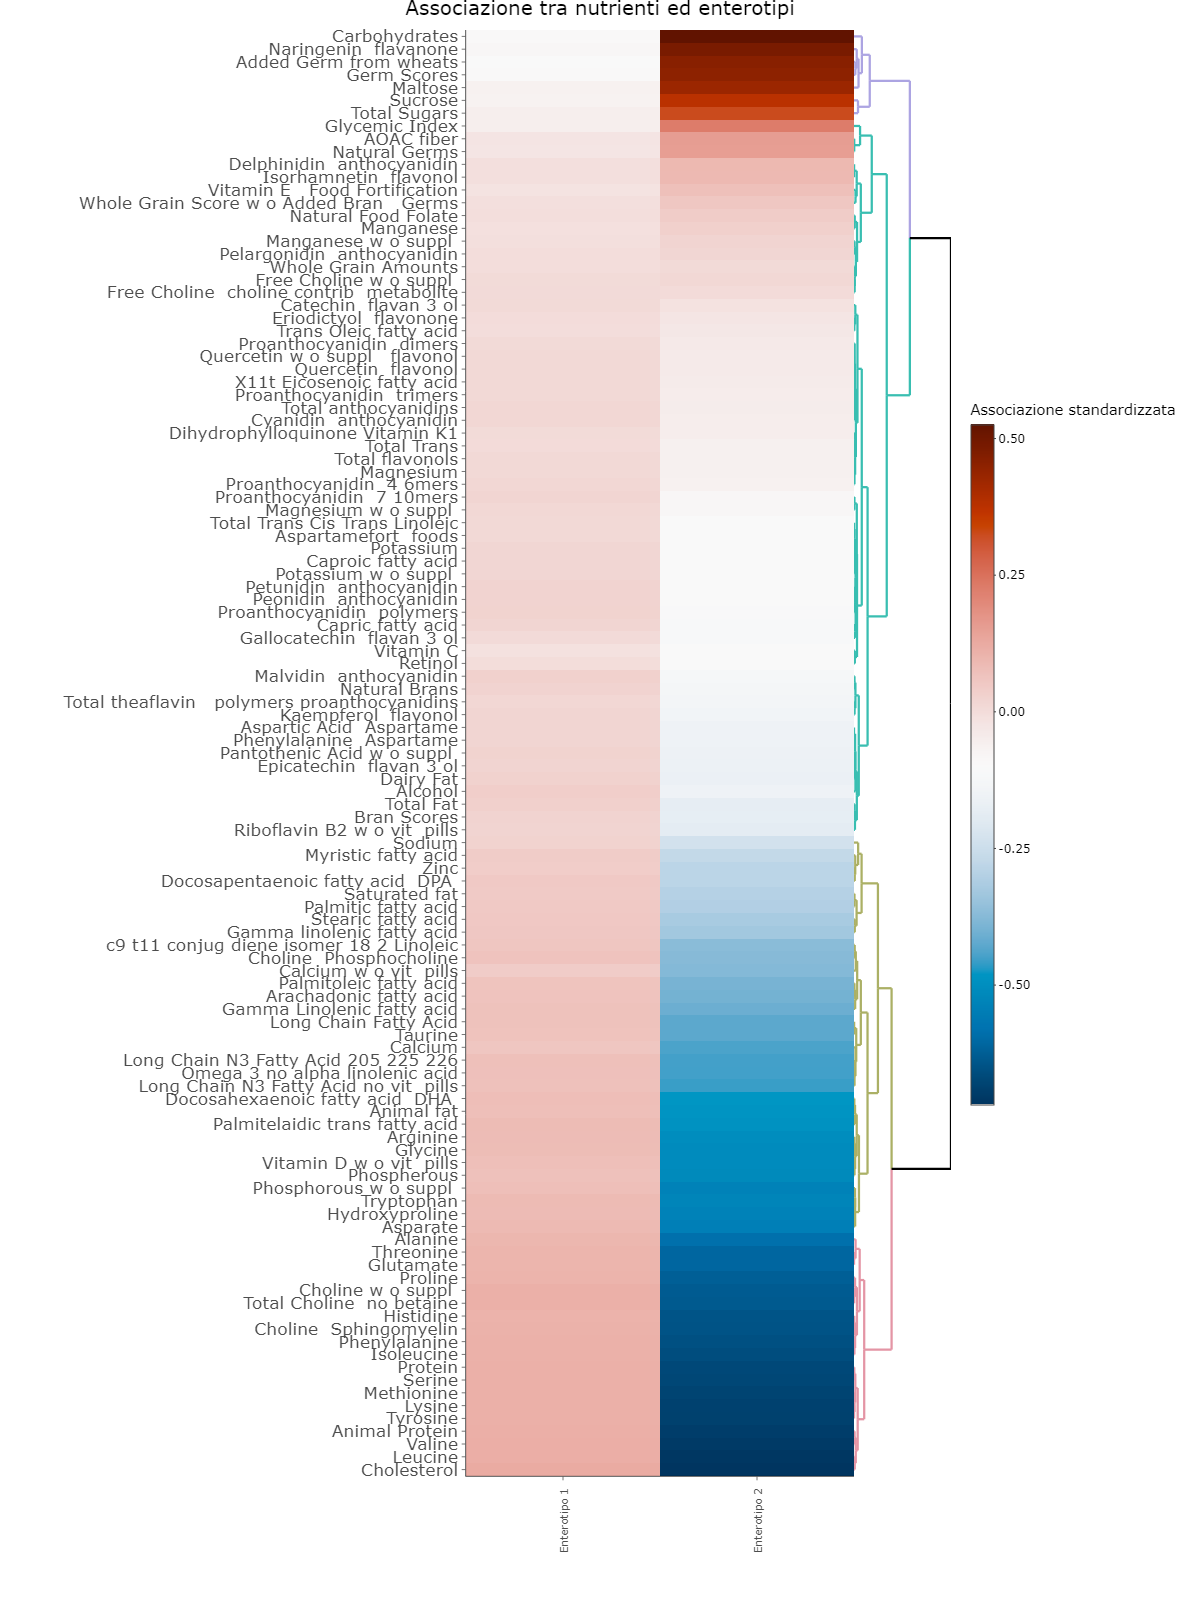
\includegraphics[width=\linewidth,keepaspectratio]{images/real_associazioni.png}
  \end{Figure}



\section{Analisi del bmi e dei regressori}
La seconda parte dello studio, si pone come obiettivo quello di sviluppare modelli capaci di prevedere la variabile y BMI, in funzione di diversi regressori. Verranno utilizzate tecniche di riduzione della dimensionalità in modo tale da poter sviluppare sia modelli lineari multivariati, sia modelli che si basano sulla procedura di Stepwise e l’uso di stimatori Lasso per poter effettuare feature selection nella fase di training. Prima di entrare nel dettaglio di tali modelli, è stata analizzata la variabile dipendente. Nella tabella successiva vengono mostrati i parametri della distribuzione del BMI:
\vspace*{1cm}
\begin{Figure}
    \centering
    \includegraphics[width=10cm,keepaspectratio]{images/stat_BMI.PNG}
  \end{Figure}
  \vspace*{1cm}
Dai risultati emerge che la media è maggiore della mediana, e questo testimonia un’asimmetria positiva nella distribuzione, concetto confermato anche dal valore della skewness pari a 1.39. Nella figura successiva viene rappresentata la distribuzione empirica della y a confronto con la normale. 
\begin{Figure}
    \centering
    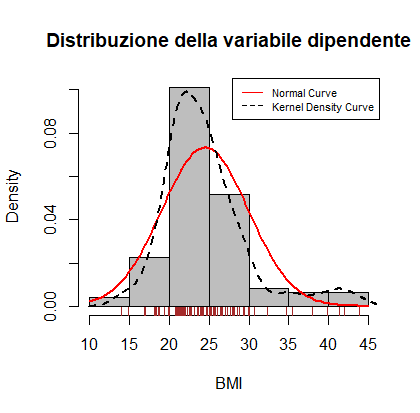
\includegraphics[width=10cm,keepaspectratio]{images/distribuzione_bmi.png}
  \end{Figure}
Dal grafico emerge che il BMI presenta, nella sua distribuzione, un’asimmetria dovuta possibilmente a degli outlier. Per effettuare un'ulteriore analisi si mostra il grafico qqplot della variabile d'interesse e viene applicato il test non parametrico Shapiro-Wilk utile per verificare la normalità della distribuzione: 
\begin{Figure}
    \centering
    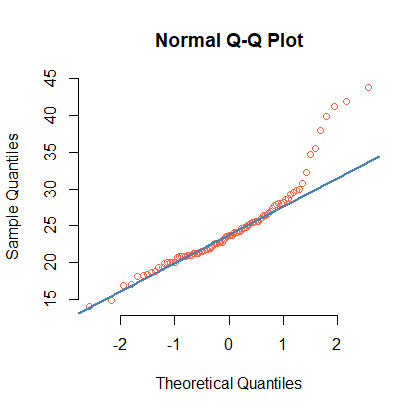
\includegraphics[width=10cm,keepaspectratio]{images/qqplot_bmi_con_outliers.png}
  \end{Figure}
Il grafico superiore assume una forma più asimmetrica che normale, a testimonianza che la coda di destra influenza la distribuzione empirica. Applicando il test Shapiro-Wilk si ottiene una statistica W pari a 0.88 e viene rigettata l’ipotesi nulla di normalità con alfa pari a 0.05. Per porre rimedio a tale problema, si fa uno studio degli outlier nella y. Esistono diverse tecniche per identificare i valori anomali, tra cui il box plot:

\begin{Figure}
    \centering
    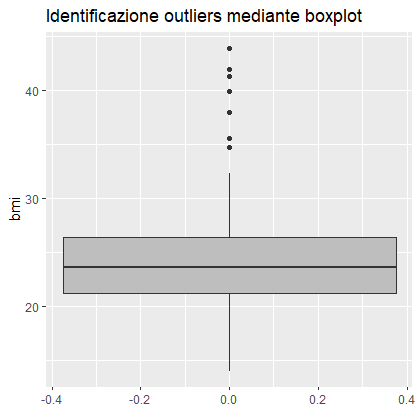
\includegraphics[width=10cm,keepaspectratio]{images/box_plot_outliers.png}
  \end{Figure}

Osservando semplicemente il boxplot si può concludere che esistono degli outlier che influenzano la distribuzione. 6 outlier sono in seguito stati rimossi. Dal grafico seguente si può osservare come tale approccio abbia corretto il problema delle code pesate:
\begin{Figure}
    \centering
    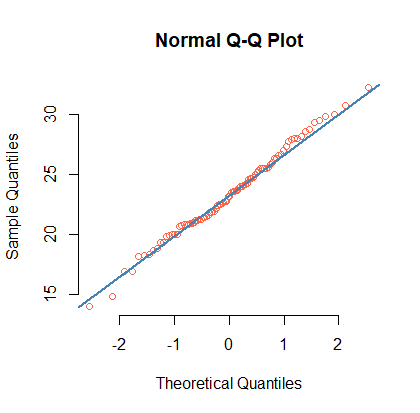
\includegraphics[width=10cm,keepaspectratio]{images/qqplot_bmi_no_outliers.png}
  \end{Figure}
Per confermare l'efficacia della rimozione degli outlier, abbiamo applicato di nuovo il test non parametrico SW, accettando l’ipotesi nulla di normalità con alfa pari a 0.05 e statistica W pari a 0.99. Inoltre, l’ipotesi di normalità degli errori è verificata.
Successivamente, è stata analizzata la distribuzione della y rispetto all’età ed il sesso in modo tale da identificare eventuali sottopopolazioni nei dati. Una volta verificata l’assunzione di normalità rispetto alla y e di varianza costante nei gruppi, abbiamo applicato il t-test a due campioni per verificare se la distribuzione della popolazione maschile differisse in modo significativo da quella femminile: il test accetta l’ipotesi nulla di uguaglianza, in media, tra le due popolazioni per alfa pari a 0.05. Mostriamo il grafico della distribuzione della y rispetto al sesso: 
\begin{Figure}
    \centering
    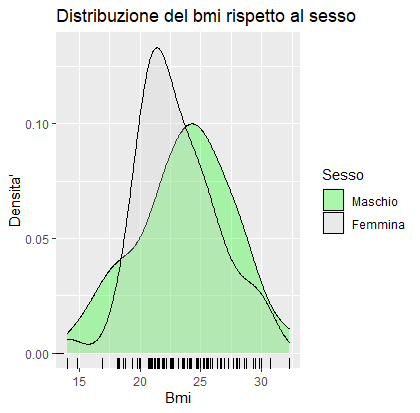
\includegraphics[width=10cm,keepaspectratio]{images/distribuzione_sesso_bmi.png}
  \end{Figure}
Un’altra variabile interessante è quella legata all’età dei pazienti. Dopo aver discretizzato l’età in 2 intervalli basati sui quantili della distribuzione, si è applicato il test Chi-quadro per verificare un'eventuale dipendenza tra le varie fasce di età e il BMI. I risultati ottenuti evidenziano che non esiste una stretta dipendenza tra l’età e la variabile y, e per questo si accetta l’ipotesi nulla di indipendenza con alfa pari a 0.05.
\begin{Figure}
    \centering
    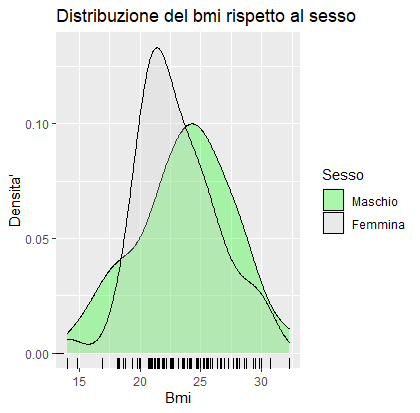
\includegraphics[width=10cm,keepaspectratio]{images/distribuzione_sesso_bmi.png}
  \end{Figure}

Dal grafico superiore, si nota come la fascia di età degli adulti tenda ad avere un BMI più alto rispetto ai giovani. Nella figura successiva, sono mostrate le correlazioni di Spearman tra BMI e le componenti principali dei batteri, dei nutrienti e sesso ed età. 
\begin{Figure}
    \centering
    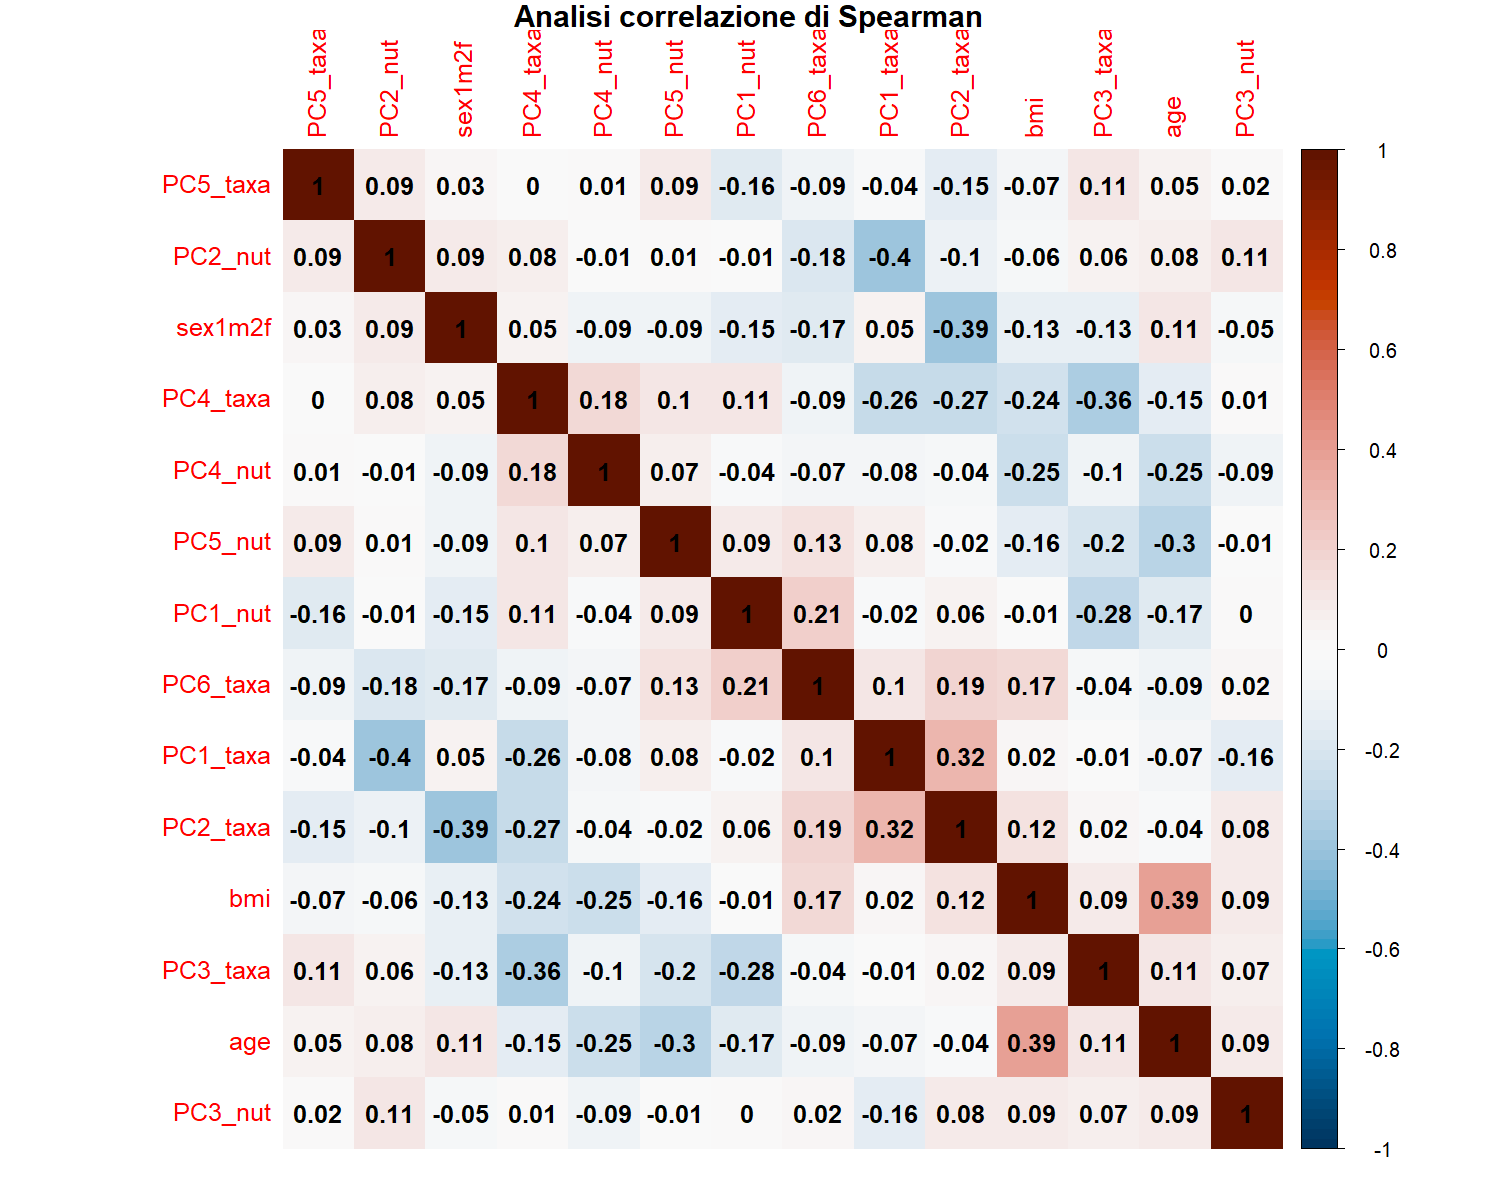
\includegraphics[width=16cm,keepaspectratio]{images/corr_plot_regressori.png}
  \end{Figure}

Si indagano le collinearità tra i regressori. Dal grafico delle correlazioni e dagli indicatori VIF e TOL si evince l'assenza di multicollinearità.


\section{Modelli}
 Per quanto riguarda il task di previsione del BMI, è stato svolto uno studio comparativo tra diversi modelli basandosi su due metriche: RMSE e R-squared adjusted. In totale, sono stati sviluppati 6 modelli con diversi regressori di input. L’analisi è strutturata in due parti: valutazione delle metriche in 10-folds CV, in modo tale da fornire dei risultati più parsimoniosi e generare dei possibili intervalli di confidenza, e il confronto finale, dei diversi modelli, valutando la previsione fatta sul test set. 
\subsection{Modello lineare 1} 
Il primo modello scelto si basa sulle prime 6 componenti principali dei batteri, l’età, il sesso e il cluster identificato dagli enterotipi: 
I coefficienti significativi di questo modello sono: B0,B4, B7, B8 per un alfa pari a 0.05. Il test F sul modello è significativo per un alfa pari a 0.05. 
\\
\\
$bmi = \beta_0 \:+\: \beta_1 PC1taxa\: +\: \beta_2 PC2taxa \:+\: \beta_3 PC3taxa\: +\: \beta_4 PC4taxa \: +\: \beta_5 PC5taxa \:+\: \beta_6 PC6taxa\: +\: \beta_7 age\: +\: \beta_8 sex \:+\: \beta_9 cluster\: +\: \epsilon$
\\
\\

\subsection{Modello lineare 2}
I regressori utilizzati per questo modello sono le prime 5 componenti principali dei nutrienti, l’età, il sesso e il cluster: 
I coefficienti significativi di questo modello sono: B0,B6, B7 per un alfa pari a 0.05. Il test F sul modello è significativo per un alfa pari a 0.05. 
\\
\\
$bmi = \beta_0 \:+\: \beta_1 PC1nutrients\: +\: \beta_2 PC2nutrients \:+\: \beta_3 PC3nutrients\: +\: \beta_4 PC4nutrients \: +\: \beta_5 PC5nutrients \: +\: \beta_6 age\: +\: \beta_7 sex \:+\: \beta_8 cluster\: +\: \epsilon$
\\
\\
\subsection{Stepwise regression: Forward vs Backward}
Poichè il numero di regressori p è maggiore del numero di osservazioni n, si deve ridurre la dimensionalità dei regressori. Procedure come best subset selection potrebbero produrre risultati migliori, a discapito del tempo computazionale. In questo caso, p è talmente elevato che non permette di provare tutte le combinazioni. Per tale motivo, è stata utilizzata la procedura stepwise su un dataset aggregato sulla tassonomia 6, componenti principali dei nutrienti e le variabili demografiche. In questo caso, sono stati valutati 46 regressori differenti.  Mostriamo i risultati ottenuti dalla procedura forward e backward con 10 fold in cross validation. Gli intervalli di confidenza al 95\%, per la metrica RMSE, sono stati generati sulla base della seguente formula:
$$RMSE_{meancv} \pm 1.96\times ((1/\sqrt{k})sd(Err^{-1}, ... , Err^{-k}))$$


\begin{Figure}
    \centering
    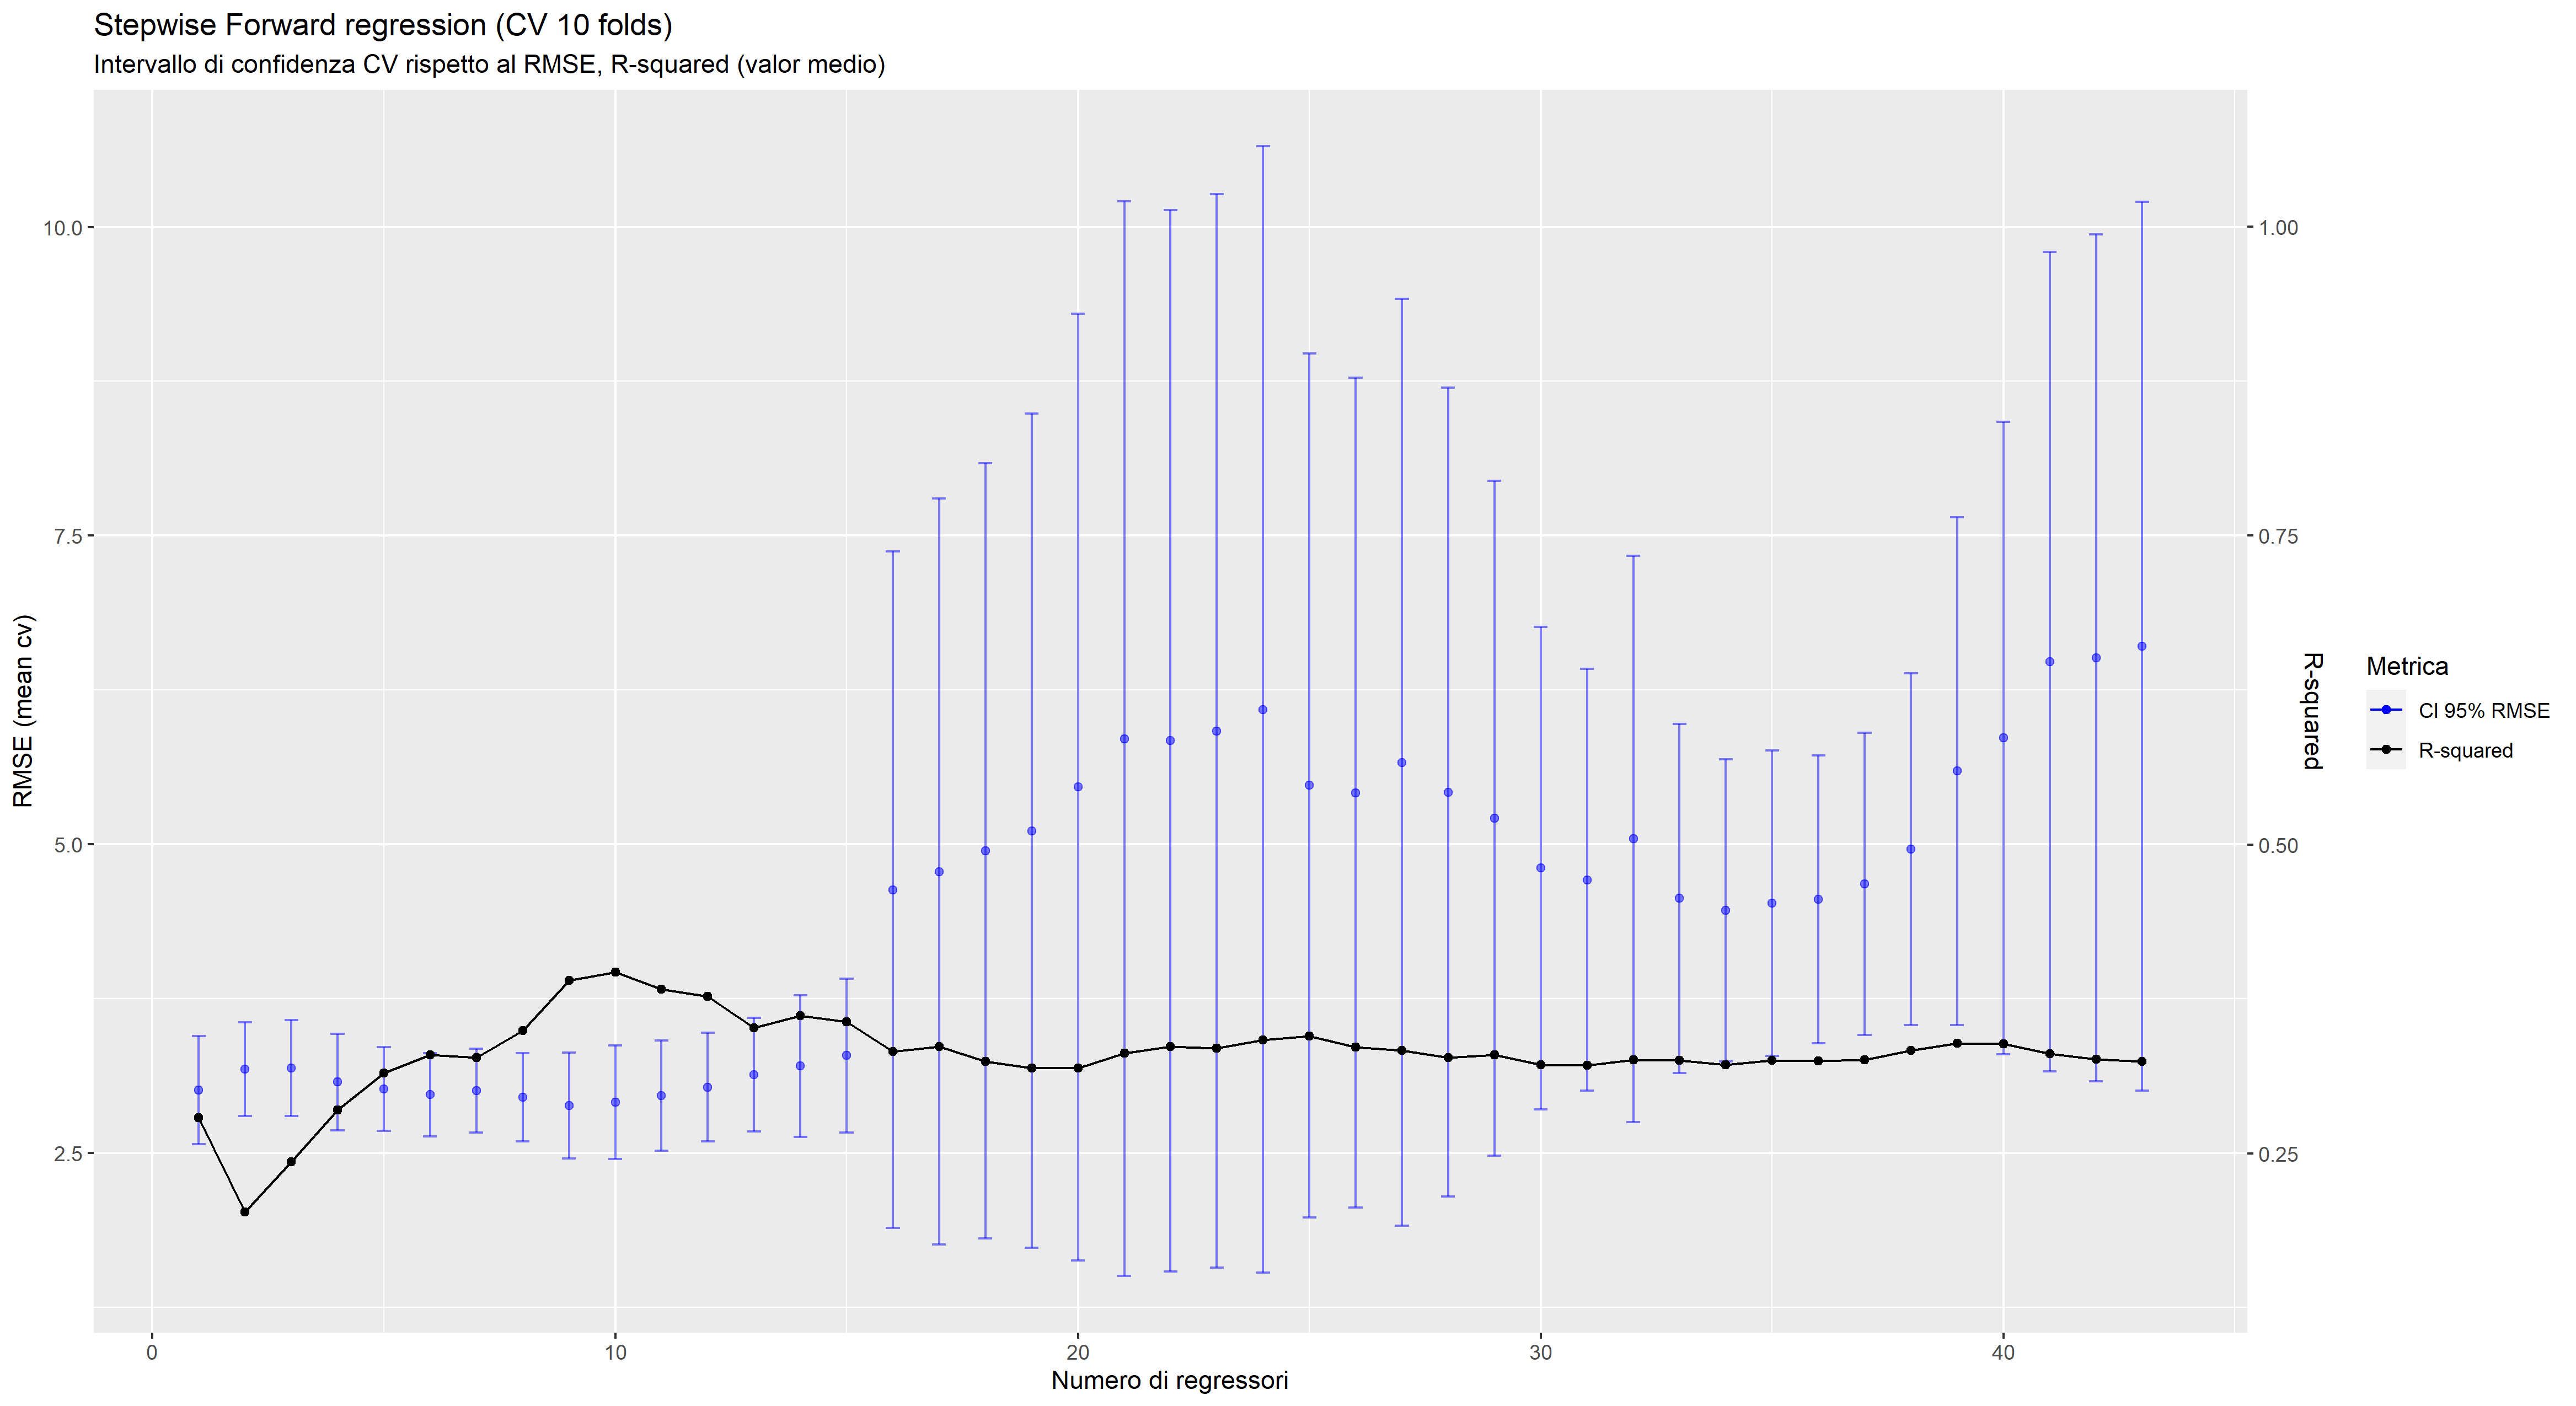
\includegraphics[width=17cm,keepaspectratio]{images/ci_stepwise_forward.png}
  \end{Figure}
\begin{Figure}
    \centering
    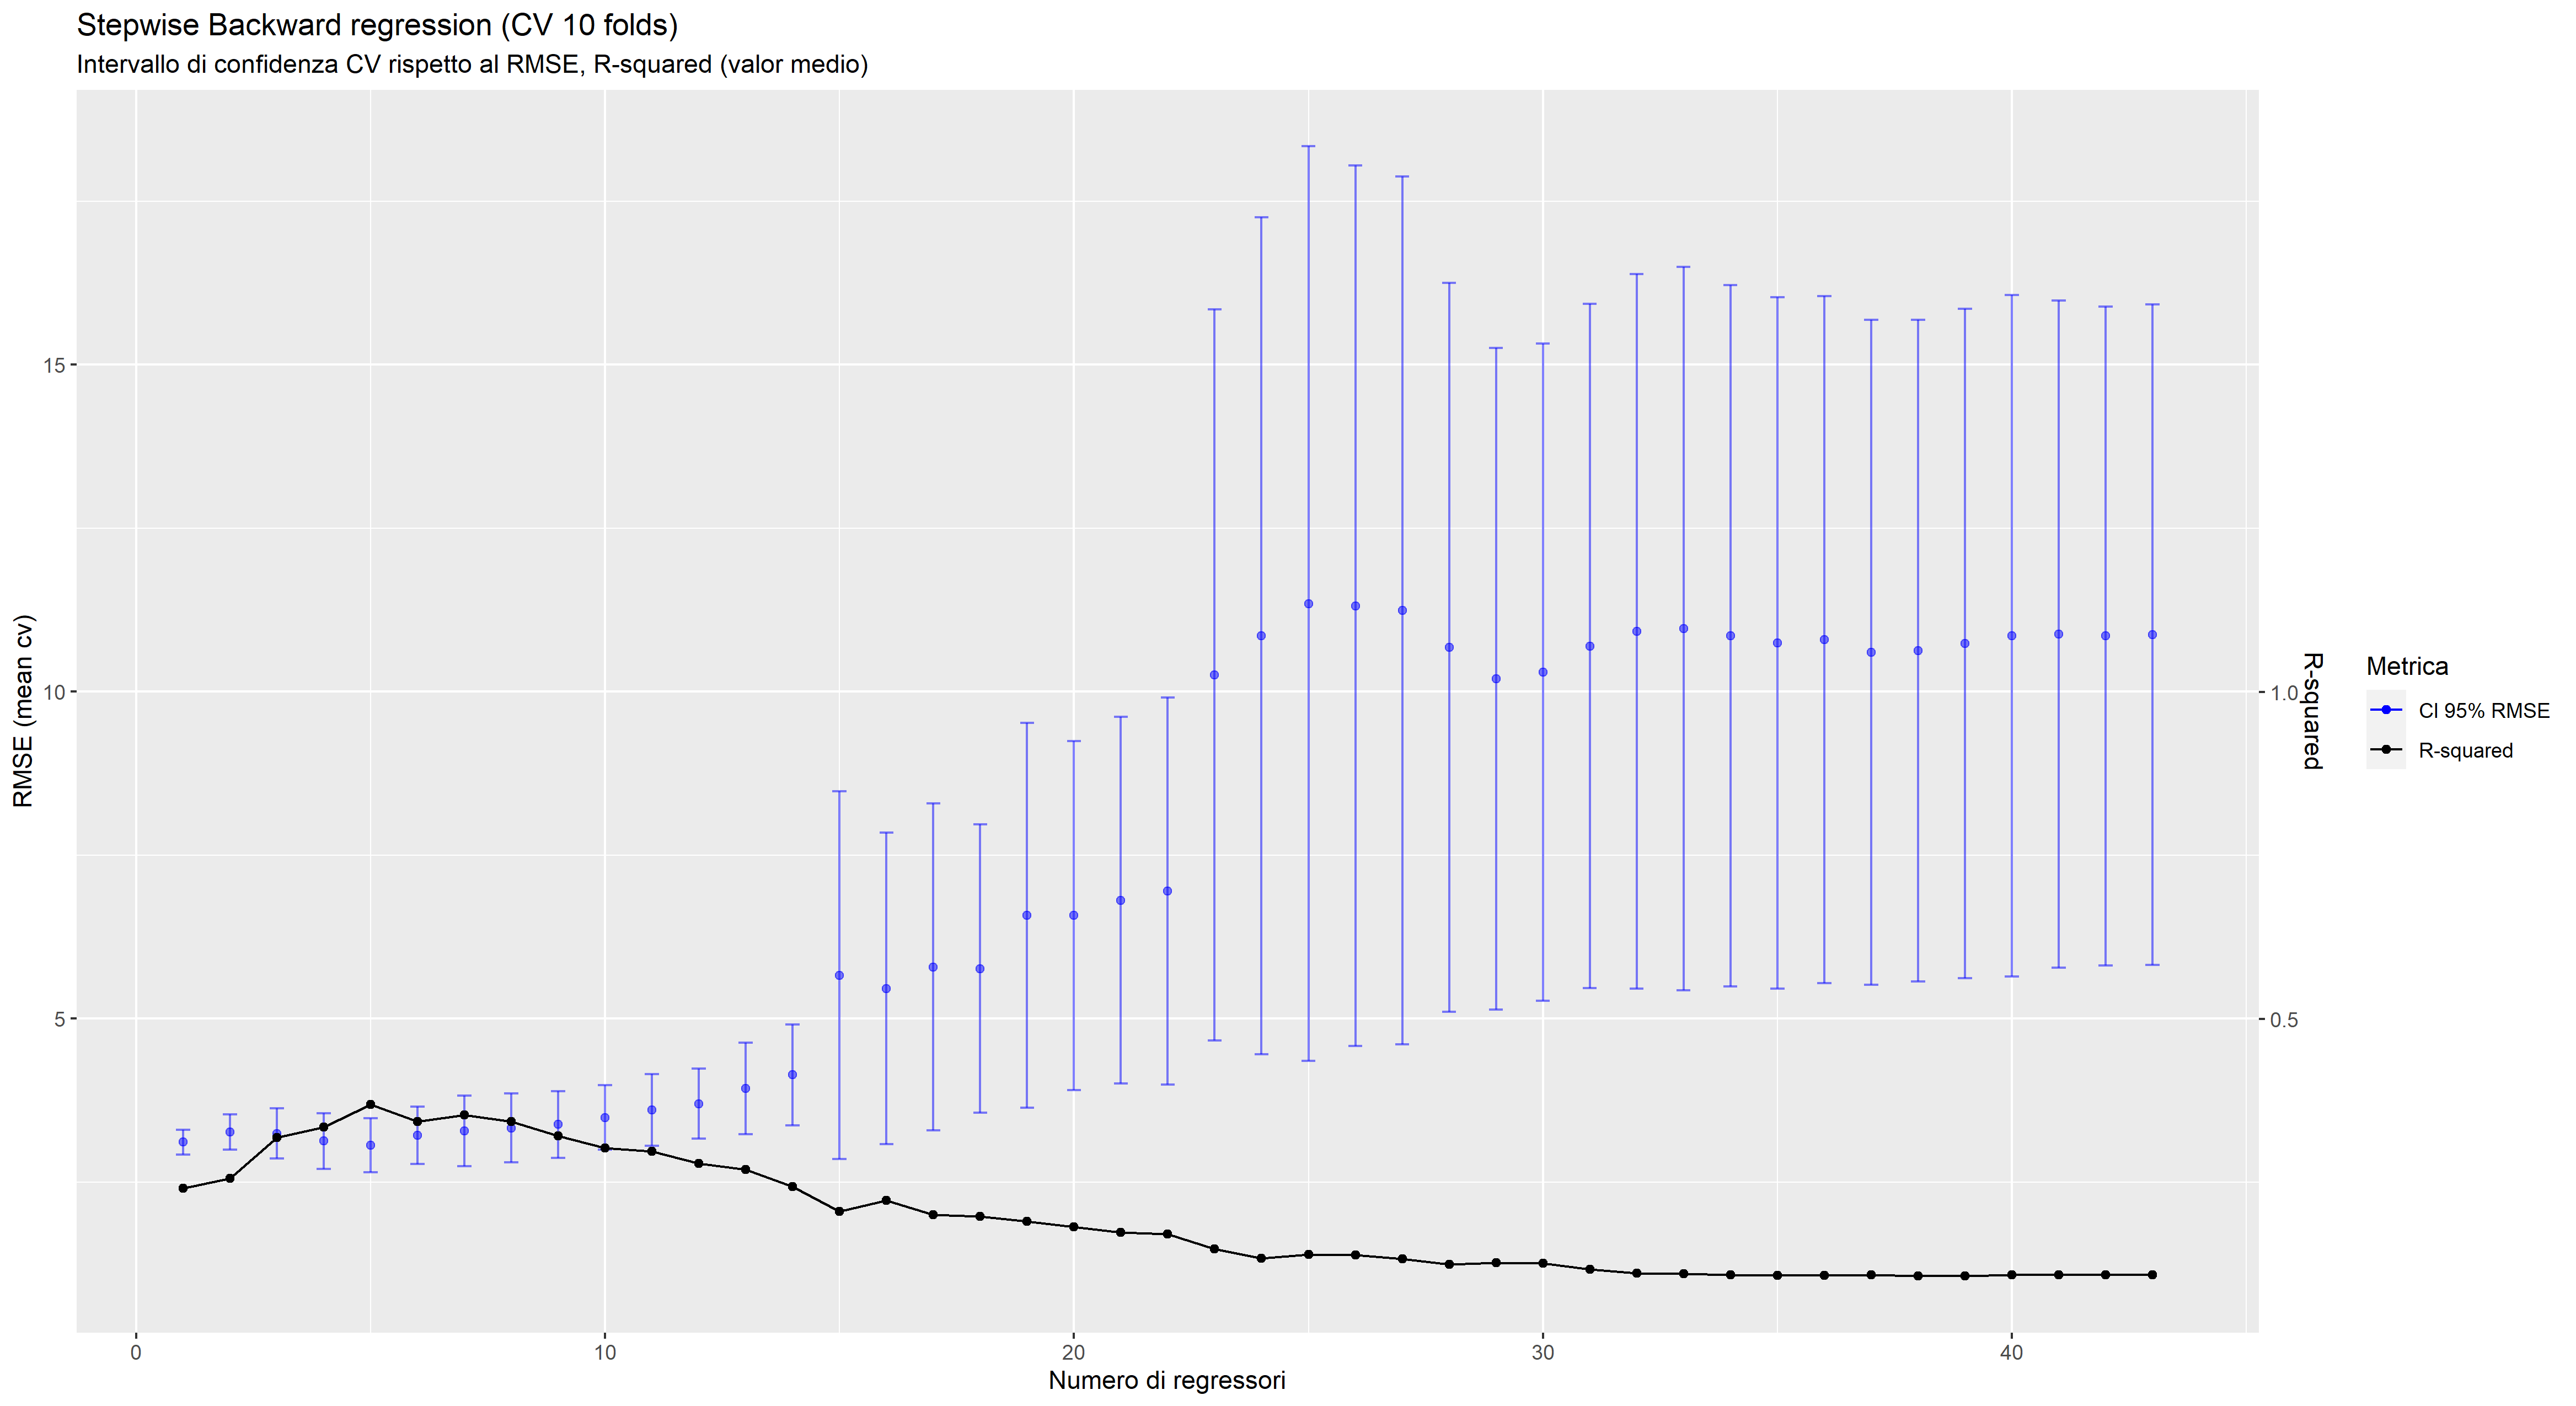
\includegraphics[width=17cm,keepaspectratio]{images/ci_stepwise_backward.png}
  \end{Figure}

Da come si evince dalle due figure, la procedura stepwise forward produce dei risultati migliori rispetto alla backward. Infatti, riesce  a produrre un modello con valori migliori di R-squared e minor numeri di regressori. Tuttavia, osservando gli intervalli di confidenza per modelli con un numero di regressori inferiore (fino a 10), non vi è una differenza significativa. Pertanto, è stato scelto il modello con 9 regressori generato dalla procedura stepwise forward. Segue l'equazione del modello. 
\\
\\
$bmi = \beta_0 \:+\: \beta_1 Parabacteroides\: +\: \beta_2 Blautia \:+\: \beta_3 Lachnobacterium\: +\: \beta_4 Megasphaera \: +\: \beta_5 Phascolarctobacterium \: +\: \beta_6 Veilonella\: +\: \beta_7 Catenibacterium \:+\: \beta_8 age\:+\: \beta_9 sex\: +\: \epsilon$
\\
\\
\subsection{Modello lasso 1}
Per quanto riguarda il modello 1, i regressori usati sono i seguenti: tutti i nutrienti assunti dalle persone, sesso, età e cluster dell’enterotipo. Tra tutti questi, quelli risultati significativi per spiegare il BMI sono i seguenti: vitamina k1 , acido stearico, idrossiprolina, flavonoidi, pelargonidina antocianidina, sesso ed età. Tra tutti questi il regressore risultato più significativo e con coefficiente maggiore tra gli altri è proprio l’età: segno che essa influenzi molto il BMI.
Nella seguente immagine si può osservare l’andamento del RMSE con relativo intervallo di confidenza al 95\% di significatività ed $R^2$ adjusted al variare dell’iperparametro Lambda.
Il valore scelto è 0.81 dato che esso massimizza l’$R^2$ adjusted e minimizza l’RMSE sebbene esso non sia significativamente migliore di tutti gli altri lambda. 

\begin{Figure}
    \centering
    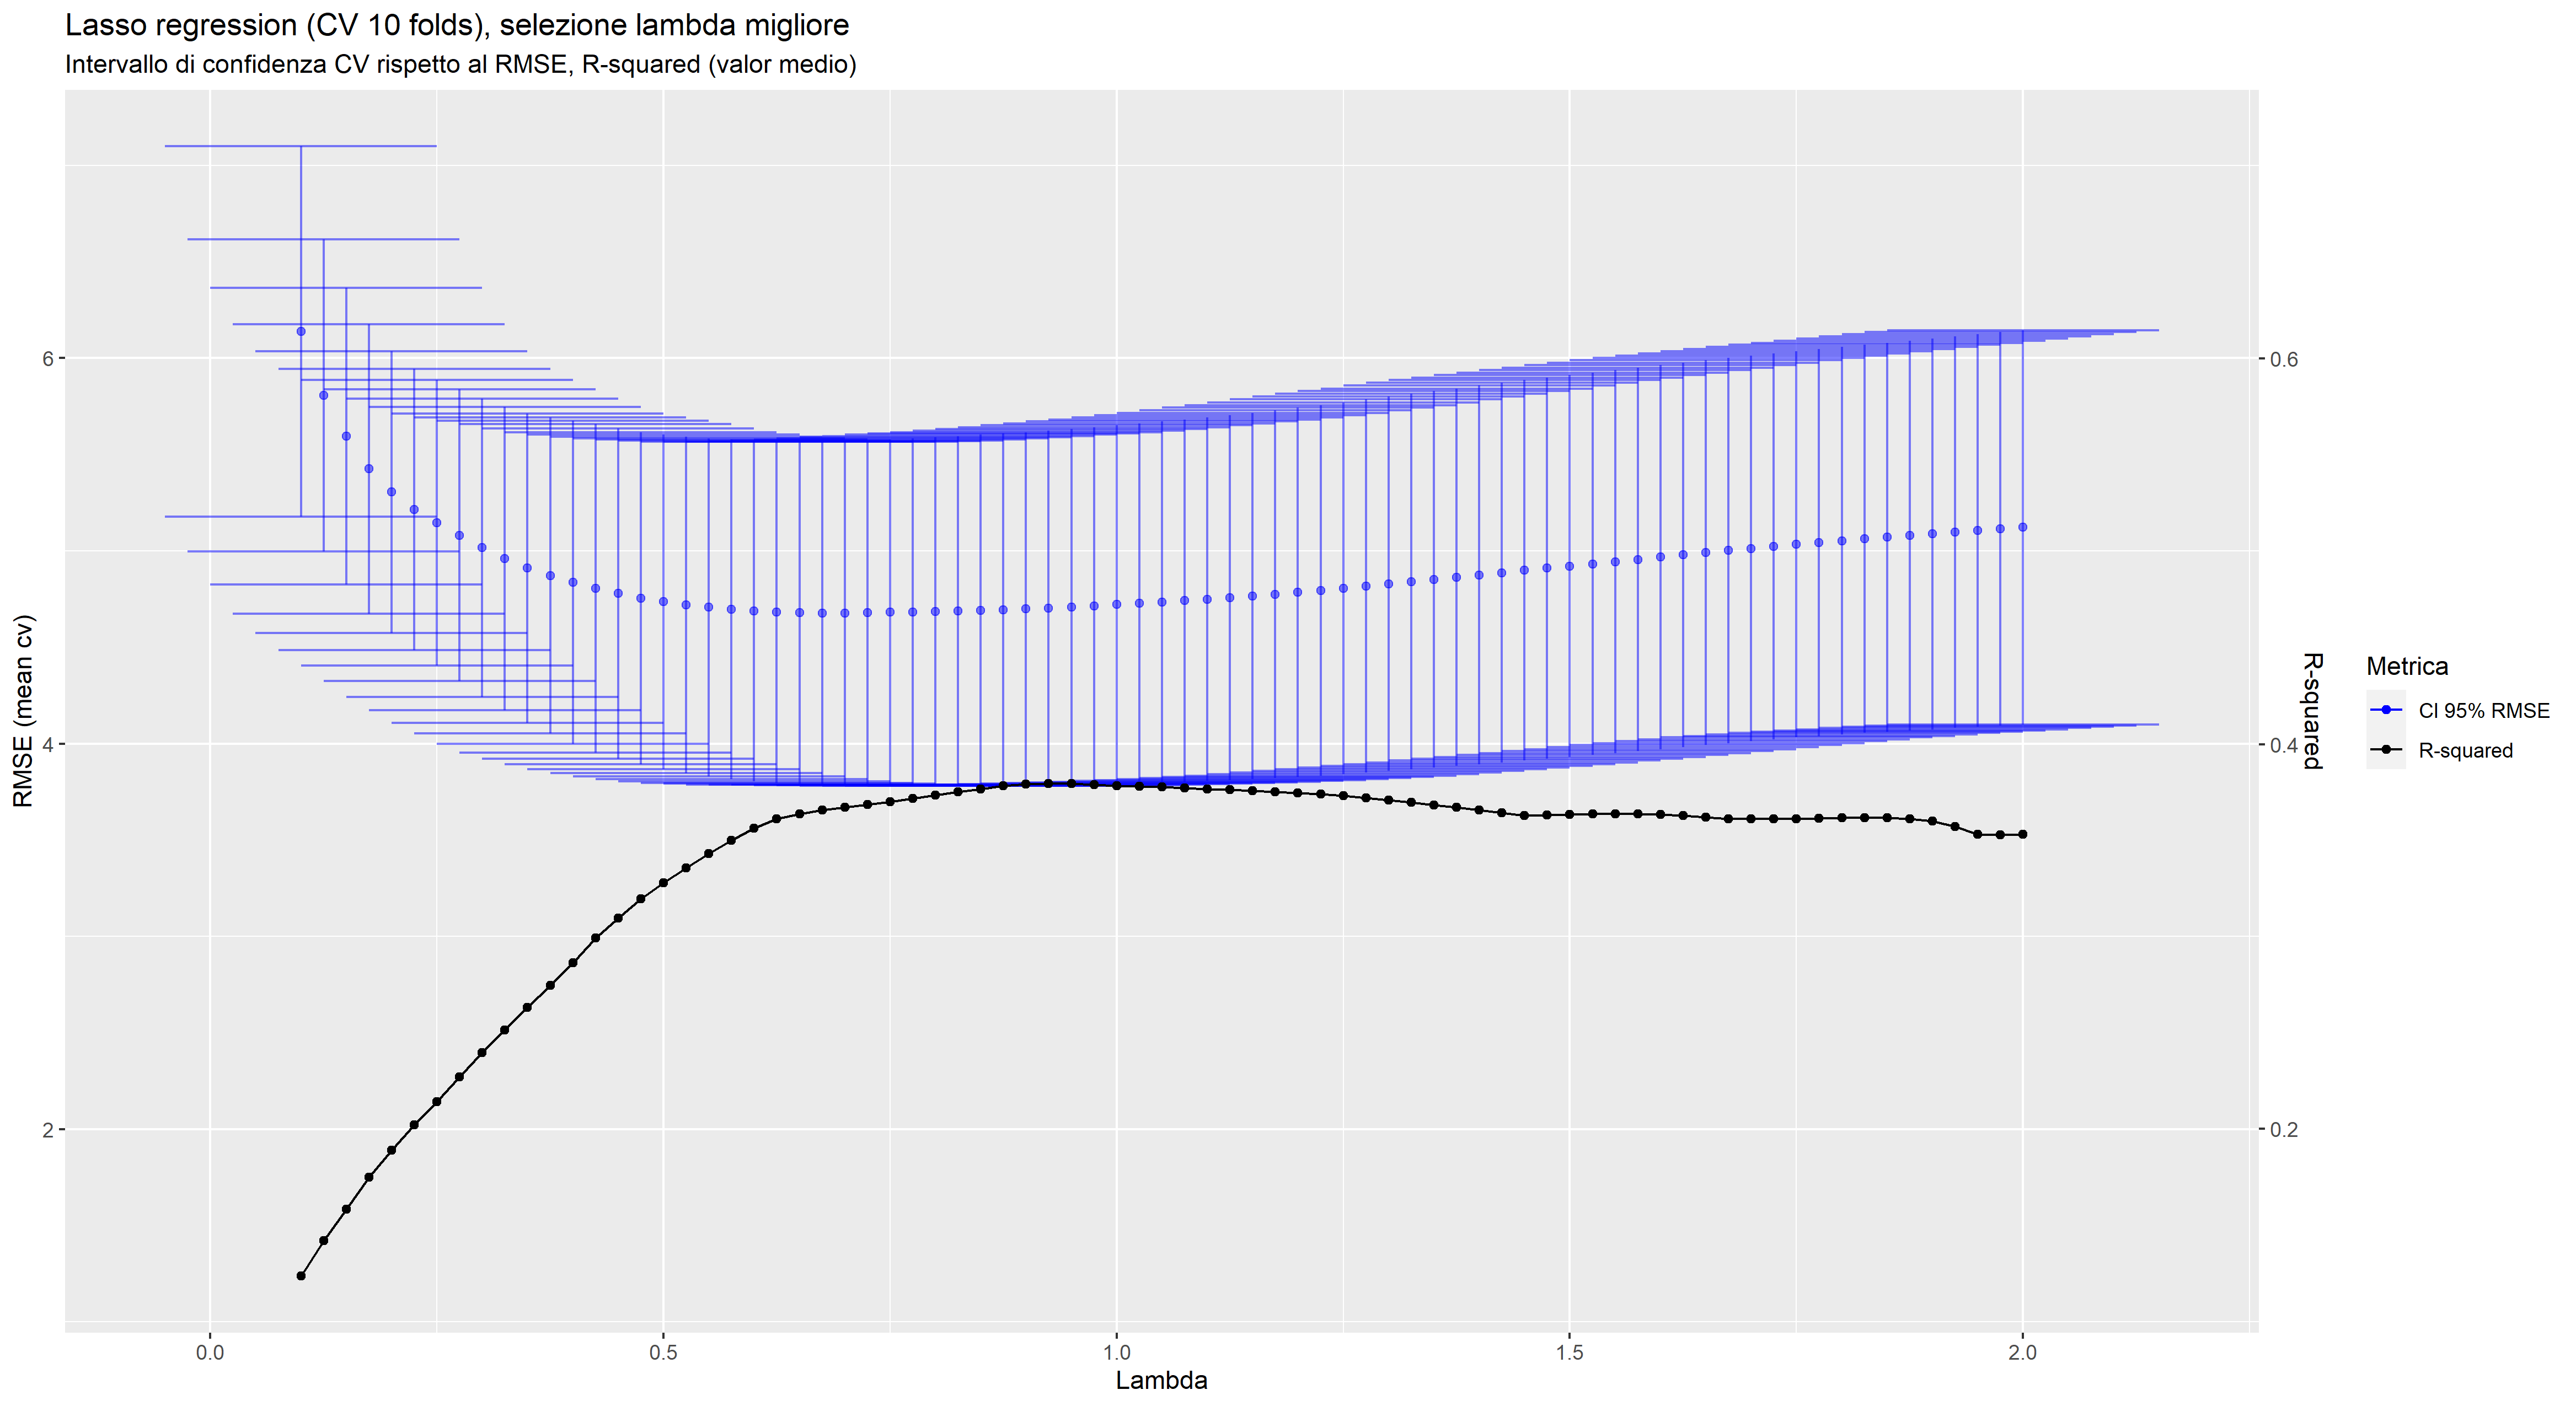
\includegraphics[width=17cm,keepaspectratio]{images/lasso_demo_nutriens_cluster.png}
  \end{Figure}
\subsection{Modello lasso 2}
Per il modello 2, i regressori usati sono i seguenti: batteri, sesso, età e cluster dell’enterotipo delle persone. Tra tutti questi, quelli risultati significativi per spiegare il BMI sono i seguenti: Megasphaera, sesso ed età.
Nella seguente immagine si può osservare l’andamento del RMSE con relativo intervallo di confidenza al 95\% di significatività ed $R^2$ adjusted al variare dell’iperparametro Lambda.
Il valore scelto è 0.70 dato che esso massimizza l’$R^2$ adjusted e minimizza l’RMSE sebbene esso non sia significativamente migliore di tutti gli altri lambda. 

\begin{Figure}
    \centering
    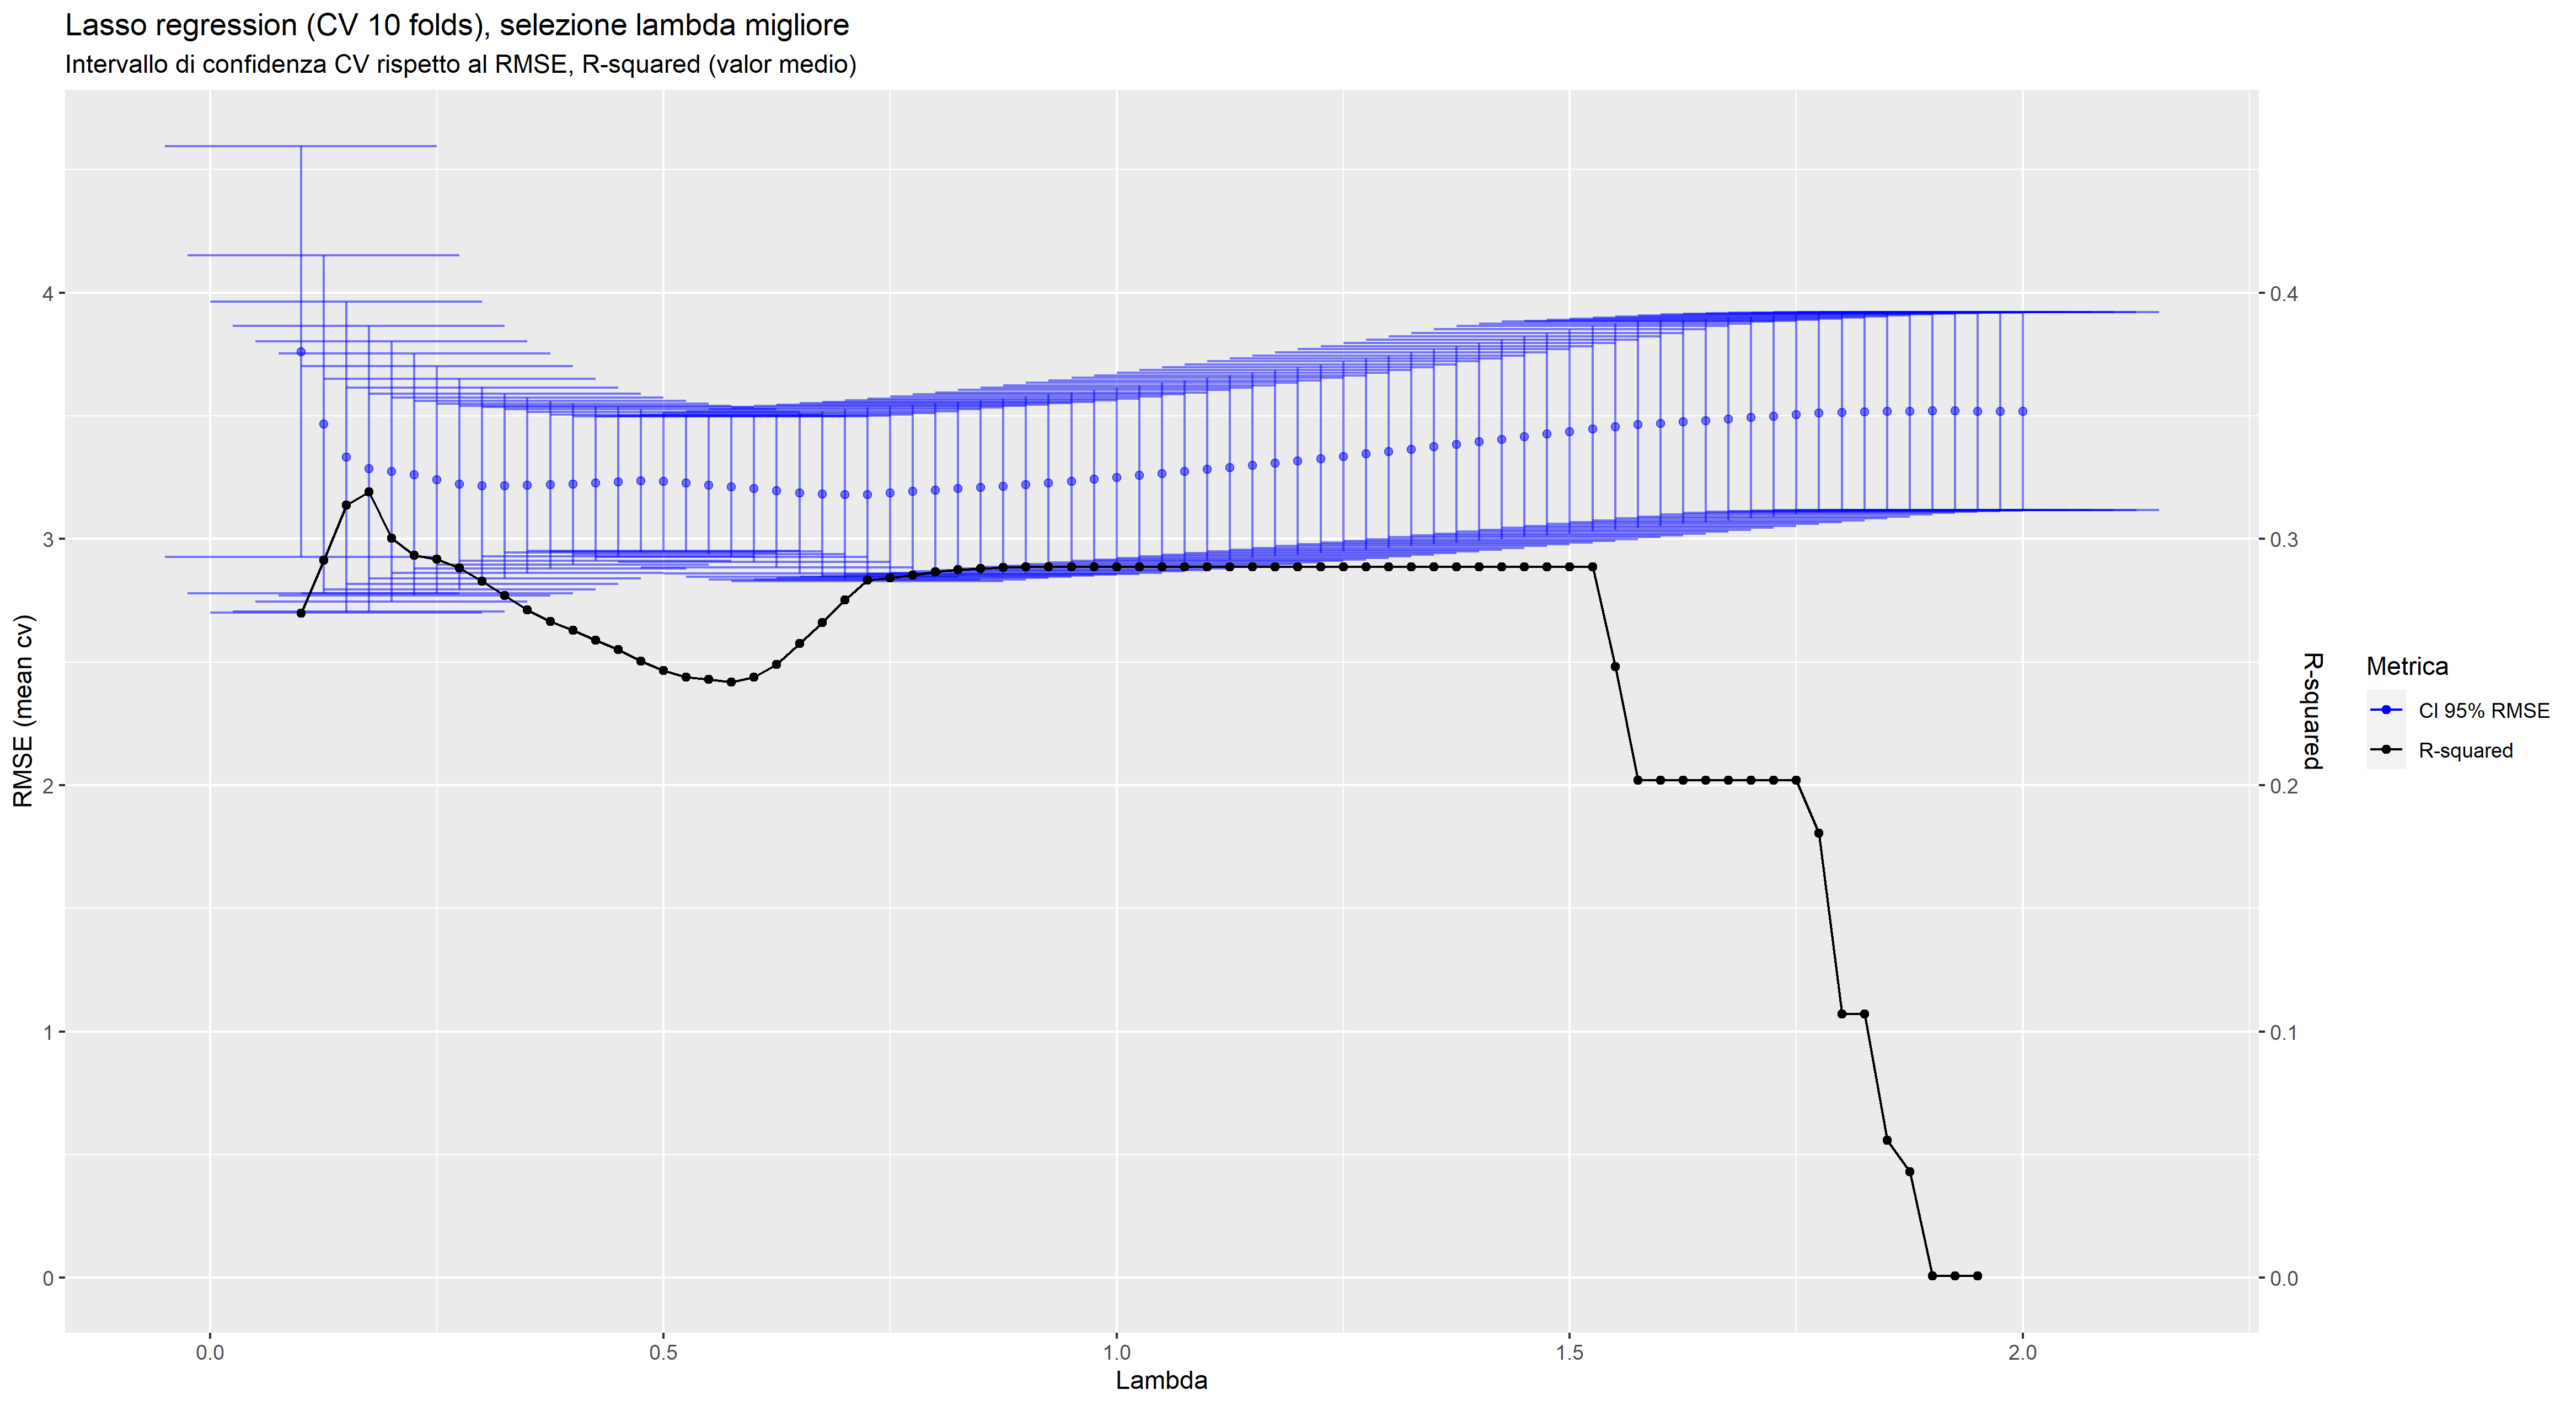
\includegraphics[width=17cm,keepaspectratio]{images/lasso_demo_37taxa_cluster.png}
  \end{Figure}
\subsection{Modello lasso 3}
Per il modello 3, sono stati usati tutti i regressori a disposizione.
Tra tutti questi, quelli risultati significativi per spiegare il BMI sono i seguenti: età, sesso e Megasphaera. Il valore di lambda scelto è 0.725 dato che esso massimizza l’$R^2$ adjusted e minimizza l’RMSE. 

\begin{Figure}
    \centering
    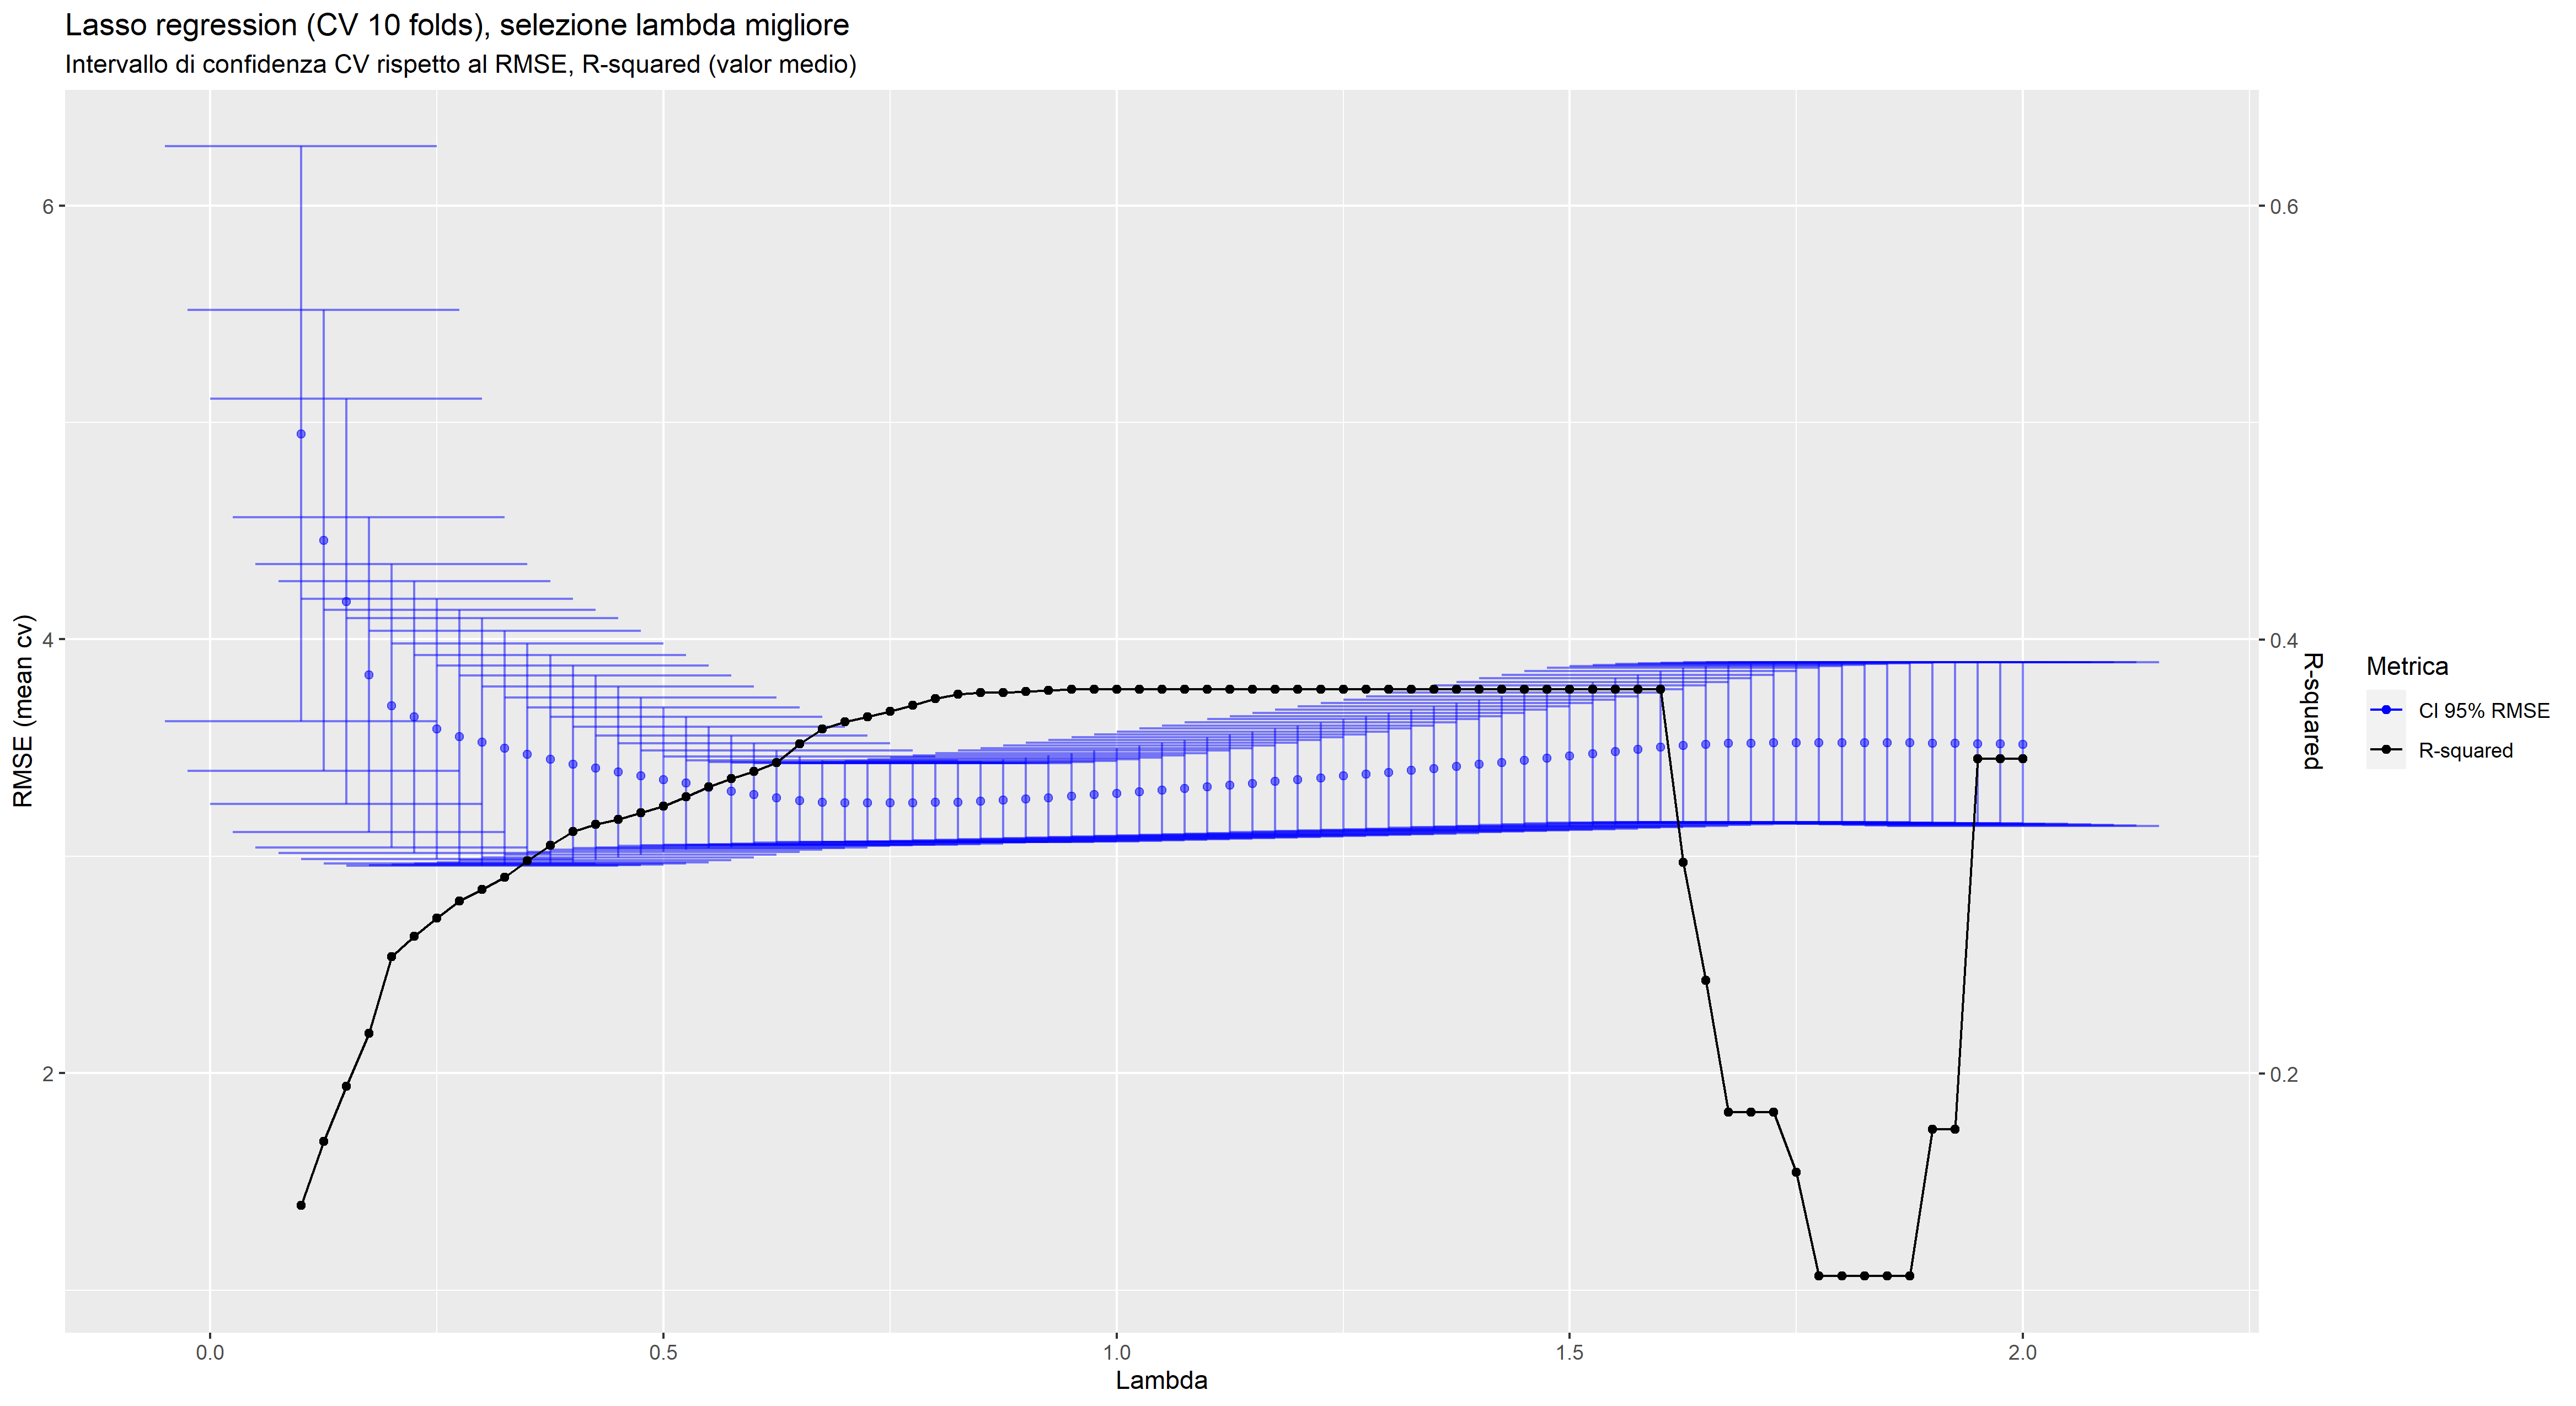
\includegraphics[width=17cm,keepaspectratio]{images/lasso_demo_37taxa_nutriens_cluster.png}
  \end{Figure}
Risultati dei modelli: 
Una volta identificati i diversi modelli, sono stati analizzati i risultati ottenuti mediante la cross-validation: 

\begin{Figure}
    \centering
    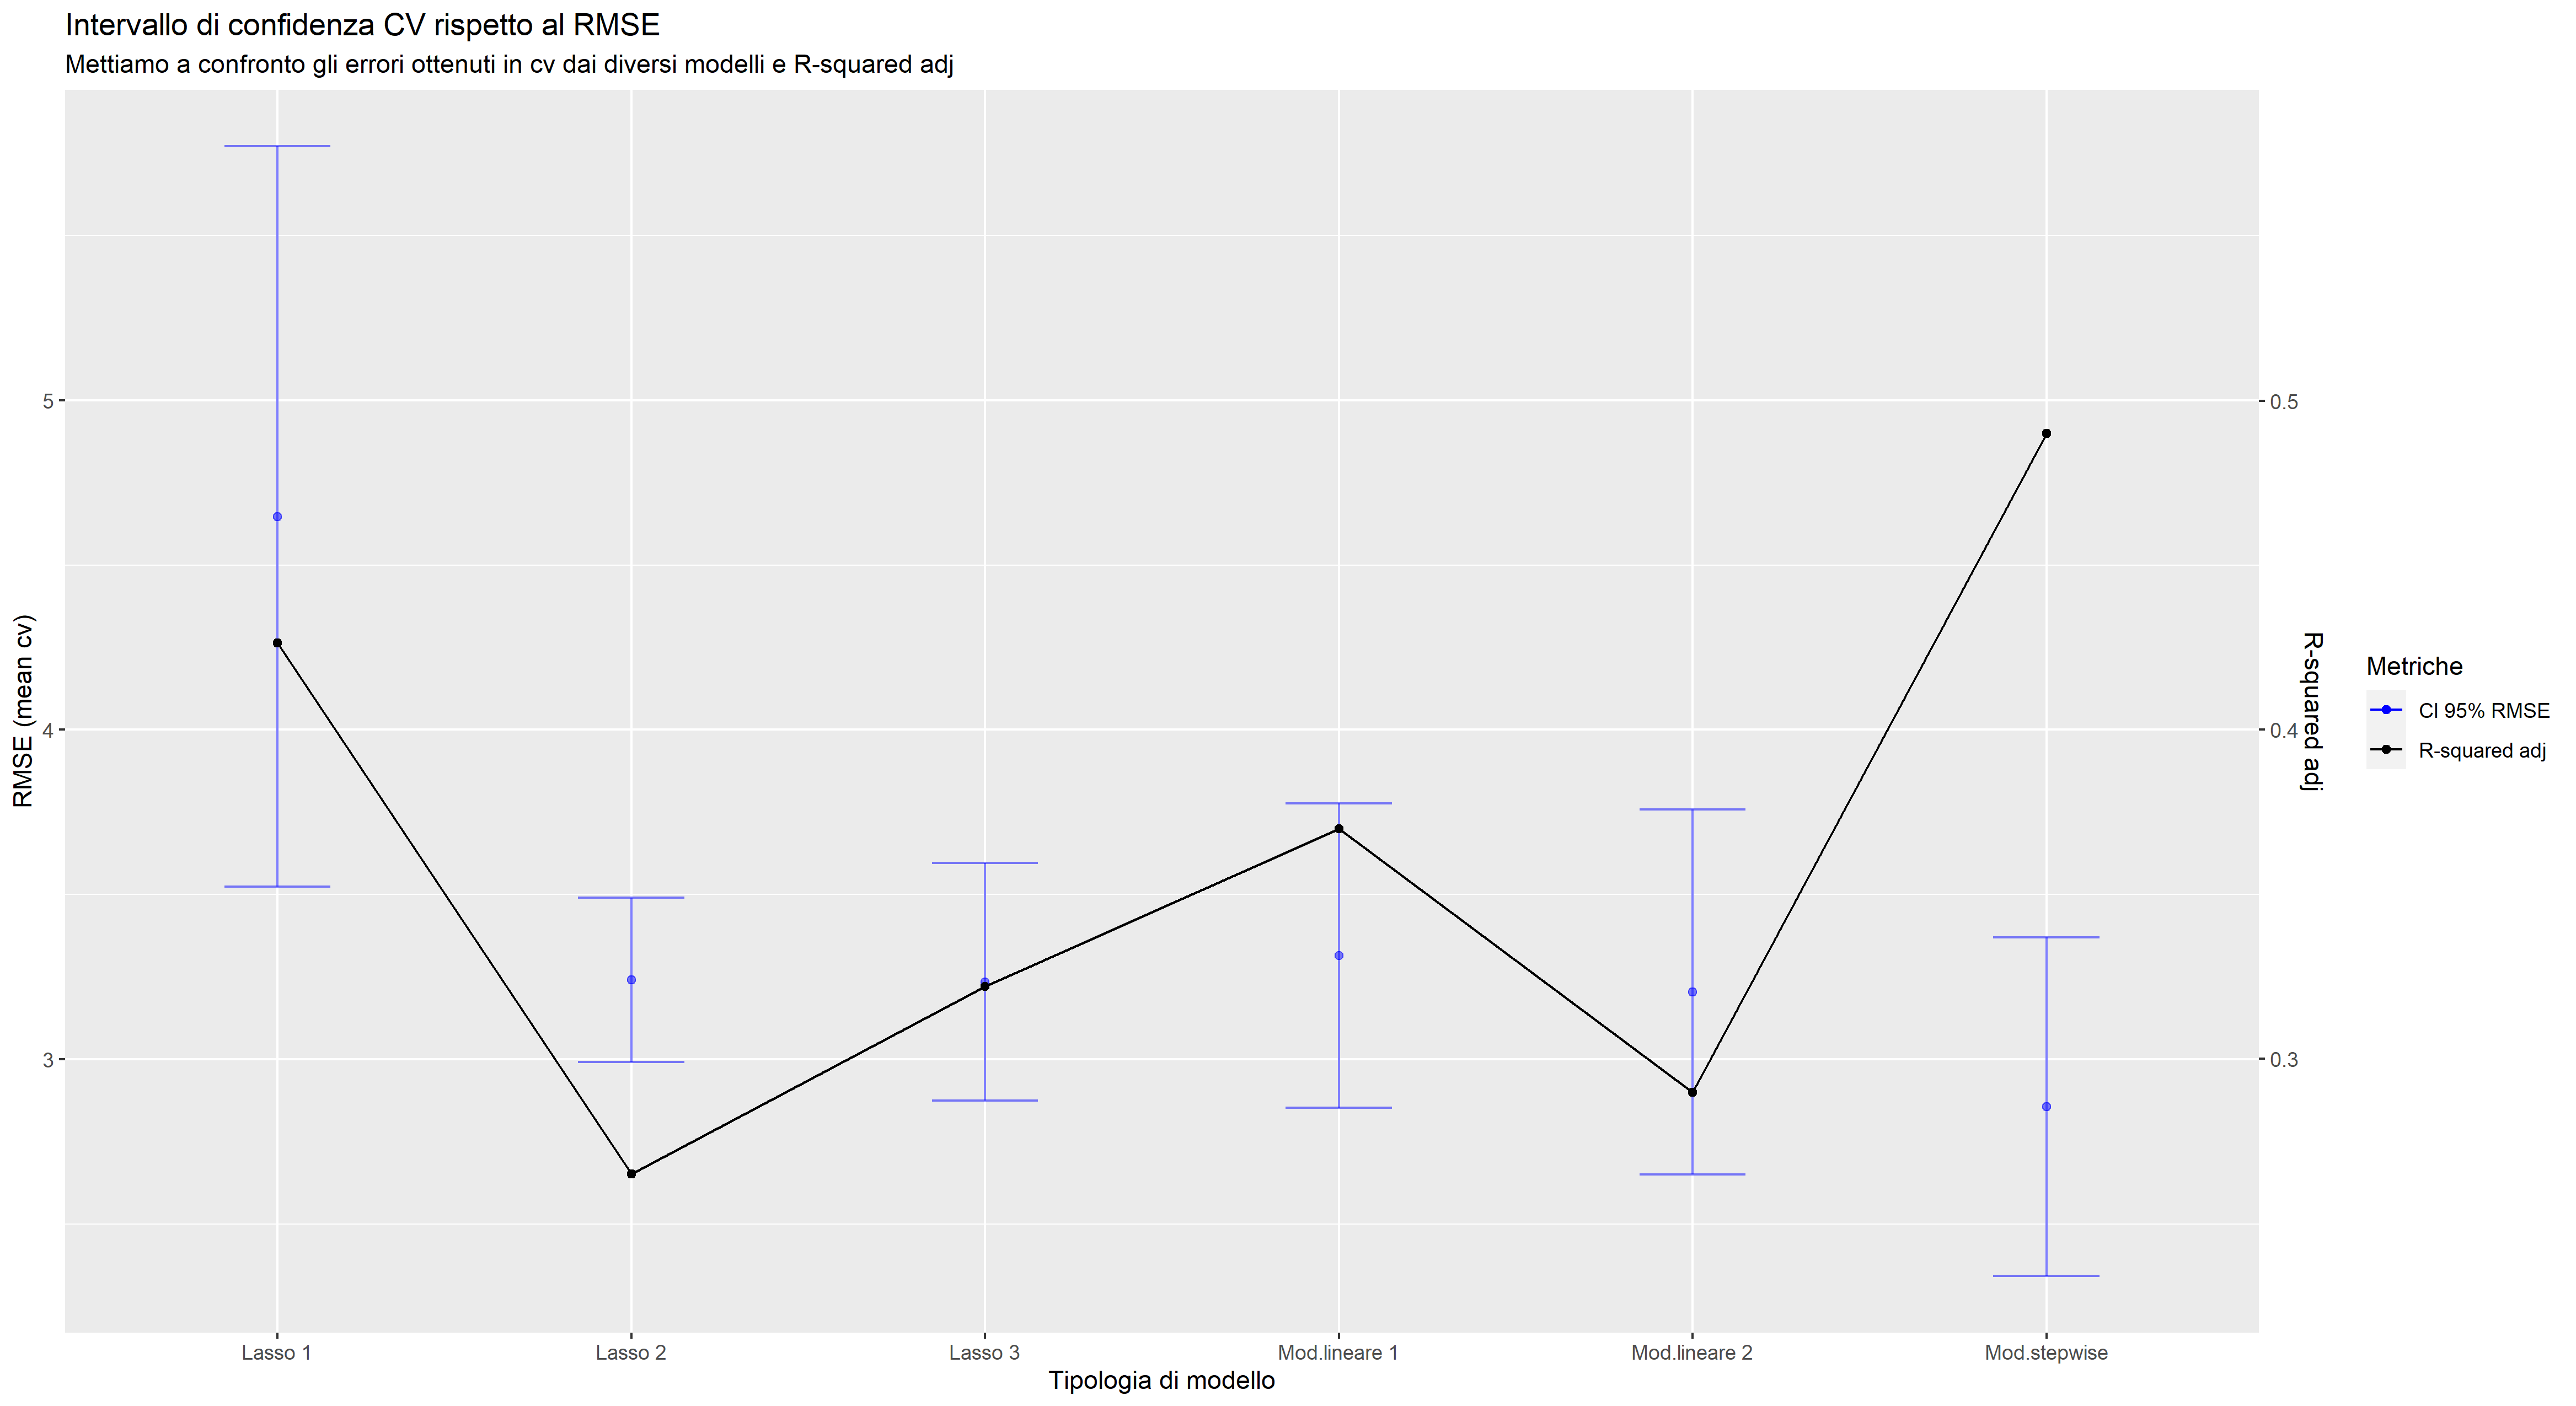
\includegraphics[width=17cm,keepaspectratio]{images/confronto_tutti_i_modelli.png}
  \end{Figure}

Nella figura superiore, si confrontano i modelli di regressione con stima OLS con quelli Lasso opportunamente calcolati con i migliori iper-parametri: il numero di regressori nel modello lineare e lambda per i modelli lasso.  Successivamente, per poter confrontare i modelli si è applicata la stessa procedura di training: cross validation con 10 fold. Questo ci ha permesso di generare degli intervalli di confidenza, sempre sulla base della formula **referenza**, e di identificare il modello migliore. Dal grafico è emerso che non esiste una differenza significativa tra i vari modelli, in termini di RMSE, tranne per il modello stepwise  e lasso 2 rispetto al lasso 1**cambiera. Inoltre, il modello che riesce a catturare più varianza, è sempre quello selezionato dalla procedura forward. Una volta stimati i modelli, sono state effettuate le previsioni sul test set. 
  \vspace*{1cm}
\begin{Figure}
    \centering
    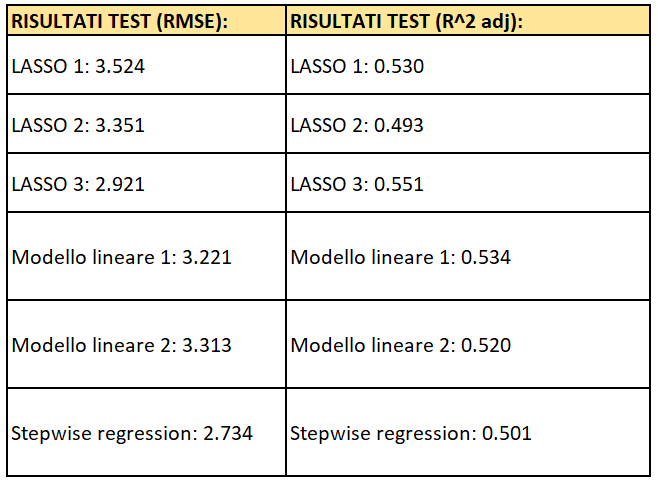
\includegraphics[width=10cm,keepaspectratio]{images/tabella_modelli.PNG}
  \end{Figure}
  \vspace*{1cm}
Dalla tabella, emerge che il modello stepwise sembrerebbe quello più affidabile in termini di risultati tra la cross validation e il test set, anche se esso è composto da sole 10 osservazioni, e quindi questo può influenzare i risultati in termini di $R^2$. Infatti, nei restanti modelli, rispetto alla Cross-validation, il coefficiente di determinazione raggiunge valori superiori, facendo emergere una presenza di underfitting nei modelli. Questo significa che tali modelli risultano essere più flessibili rispetto al test set ma più rigidi nel training set. Per questo principio sceglieremo il modello stepwise, essendo quello più parsimonioso in termini di trade off di varianza e distorsione sia per il training set sia per il test set. Questa valutazione è stata fatta rispetto al valore puntuale stimato, sarebbe interessante stimarsi anche l’intervallo di confidenza del coefficiente di determinazione, in modo tale da poter osservare la stima intervallare. Ovviamente, avendo dei valori del R-squared inferiori a 0.6, tutti i modelli non riescono a prevedere, in modo accurato, il BMI. Questo è anche dovuto dal fatto che tra i regressori e la variabile risposta, non esistono forti dipendenze tale per cui si riesce a spiegare bene l’indice di massa corporea. 

\section{Conclusioni}
Dall'analisi è emersa una forte associazione tra dieta ed enterotipo, caratterizzato dalla presenza/assenza dei batteri Bacteroides e Prevotella entrambi appartenenti al phylum Bacteroidetes. L'enterotipo con maggiore presenza di Prevotella risulta fortemente associato con diete ricche di fibre e carboidrati mentre la presenza di Bacteroides è associata con diete ricche di proteine e grassi animali. Poichè il BMI è calcolato tramite peso ed altezza è interessante valutare se le associazioni con i nutrienti ed i batteri lo influenzano. I modelli stimati evidenziano che l'età è un fattore molto influente per il BMI mentre l'enterotipo non lo è. I batteri significativi per spiegare il BMI sono Catenibacterium, Megasphaera, Parabacteroides, Blautia, Lachnobacterium, Phascolarctobacterium, Veillonella, Catenibacterium . Tra questi solo Parabacteroides appartiene al phylum Bacteroidetes mentre gli altri sono del phylum Firmicutes. I batteri del phylum, ad eccezione di Lacnobacteria, influenzano positivamente il BMI mentre  Parabacteroides negativamente. In conclusione, dal nostro studio si evince che i firmicutes sono i batteri che più influenzano la crescita del BMI.


\begin{thebibliography}{9}
\bibitem{paper} Wu, Gary D., et al. "Linking long-term dietary patterns with gut microbial enterotypes." Science 334.6052 (2011): 105-108.
\bibitem{permanova} McArdle, Brian H., and Marti J. Anderson. "Fitting multivariate models to community data: a comment on distance based redundancy analysis." Ecology 82.1 (2001): 290 297.
\bibitem{unifrac} Lozupone, Catherine, et al. "UniFrac: an effective distance metric for microbial community comparison." The ISME journal 5.2 (2011): 169 172.
\bibitem{jsd} https://bit.ly/2zs5YFv
\end{thebibliography}
\end{document}